\documentclass[11pt, a4paper, twoside, openright]{book}
%\documentclass[a4paper,11pt]{article}
\usepackage[T1]{fontenc}
\usepackage{textcomp}
\usepackage[utf8]{inputenc} %per riuscire a scrivere gli accenti
\usepackage[english]{babel} % lingua del documento
\usepackage{url} % per scrivere gli indirizzi Internet


\usepackage[top=2cm,bottom=2cm,left=2cm,right=2cm]{geometry}
%\usepackage[pdftex]{graphicx} %per poter inserire le figure

\usepackage{amssymb,amsmath,amsthm,amsfonts}

\usepackage{xspace}
\usepackage{indentfirst}
%\usepackage{subfigure}
\usepackage[small]{caption}
\usepackage{eucal}
\usepackage{eso-pic}
\usepackage{afterpage}
\usepackage{parskip}
\usepackage{listings}
\usepackage{fancyhdr}
\usepackage{cite}
\usepackage{multirow}
\usepackage{setspace}
\pagestyle{fancy} 

\usepackage{subfig}

\usepackage{amsmath}
\usepackage{amsthm} % dopo amsmath
\usepackage{amssymb}
\usepackage{booktabs}
\usepackage{caption}
%\usepackage{siunitx}
\usepackage{graphicx}
\usepackage{tabularx}
\usepackage{array,makecell}
\usepackage{enumerate}
\usepackage[export]{adjustbox}
\usepackage{verbatim}

\usepackage{tikz}
\usepackage{circuitikz}
\usepackage[qm]{qcircuit}

%Pacchetti per abstract%
\usepackage{fancyhdr}
\newenvironment{abstract}%
{\cleardoublepage%
\thispagestyle{empty}%
\null \vfill\begin{center}%
\bfseries \abstractname \end{center}}%
{\vfill\null}

%%%%%%INTESTAZIONE DELLE PAGINE NEI CAPITOLI come voglio io%%%%%%
%ROCCO%%ROCCO%%ROCCO%%ROCCO%%ROCCO%%ROCCO%%ROCCO%%ROCCO%%ROCCO%
%\pagestyle{fancy}
%
%\fancyhead[LE,RO]{\nouppercase{\slshape \rightmark}}
%\fancyhead[LO,RE]{\nouppercase{\slshape \leftmark}}
%\fancyfoot[C]{\thepage}
%ROCCO%%ROCCO%%ROCCO%%ROCCO%%ROCCO%%ROCCO%%ROCCO%%ROCCO%%ROCCO%
\pagestyle{fancy}
\fancyhf{}
\fancyhead[RE]{\ifnum\value{chapter}>0\nouppercase{\leftmark}\fi}
\fancyhead[LE]{\small\textbf{\thepage}}
\fancyhead[LO]{\nouppercase{\rightmark}}
\fancyhead[RO]{\small\textbf{\thepage}}

\renewcommand{\chaptermark}[1]{%
 \markboth{\MakeUppercase{%
 \chaptername}\ \thechapter.%
 \ #1}{}}
 
%\fancyhf{} % azzeriamo i campi
%\fancyhead[RE]{\leftmark}
%\fancyhead[LO]{\nouppercase{\rightmark}}




%%Per scrivere identità%%
\usepackage{bbold}



%%%%Box colorato%%%%
\usepackage{xcolor}
\usepackage{framed}
\definecolor{shadecolor}{rgb}{0.93, 0.93, 0.93}%{0.9, 0.89, 0.89} % platinum
%%%colore verde python%%%
\definecolor{darkgreen}{rgb}{0.0, 0.5, 0.0}
\definecolor{darkred}{rgb}{0.8, 0.0, 0.0}
\definecolor{violet}{rgb}{0.55, 0.0, 0.55}

%PYTHON CODE IN LATEX%%%%%%%%%%%%%%%%%%%%
\usepackage{listings}
\usepackage{xcolor}
 
\definecolor{codegreen}{rgb}{0,0.6,0}
\definecolor{codegray}{rgb}{0.5,0.5,0.5}
\definecolor{codepurple}{rgb}{0.58,0,0.82}
\definecolor{backcolour}{rgb}{0.95,0.95,0.92}
\definecolor{commentcolour}{rgb}{0.43,0.63,0.65}
 
%\lstdefinestyle{mystyle}{ %Stile python code
%    backgroundcolor=\color{backcolour},   
%    commentstyle=\color{codegreen},
%    keywordstyle=\color{magenta},
%    numberstyle=\tiny\color{codegray},
%    stringstyle=\color{codepurple},
%    basicstyle=\ttfamily\footnotesize,
%    breakatwhitespace=false,         
%    breaklines=true,                 
%    captionpos=b,                    
%    keepspaces=true,                 
%    numbers=left,                    
%    numbersep=5pt,                  
%    showspaces=false,                
%    showstringspaces=false,
%    showtabs=false,                  
%    tabsize=2
%}
% 
%\lstset{style=mystyle}

\lstdefinestyle{mystyle}{ %Stile python code
    backgroundcolor=\color{shadecolor},   
    commentstyle=\color{commentcolour},
    keywordstyle=\color{darkgreen},
    numberstyle=\tiny\color{codegray},
    stringstyle=\color{darkred},
    basicstyle=\ttfamily\footnotesize,
    breakatwhitespace=false,         
    breaklines=true,                 
    captionpos=b,                    
    keepspaces=true,                 
    numbers=left,                    
    numbersep=5pt,                  
    showspaces=false,                
    showstringspaces=false,
    showtabs=false,                  
    tabsize=2
}
 
\lstset{style=mystyle}




%%%Blocco immagine nella posizione che si vuole%%%
\usepackage{float} %poi bisogna usare un \begin{figure}{H}



%%%%%indent%%%
\setlength{\parindent}{15pt}
\setlength{\parskip}{0pt}



%%%%%circuito secondo capitolo %%%%%%%%%
\usetikzlibrary{fit}
% \sl è una variabile definita per automatizzare la procedura di posizionamento con le coordinate e rendere migliori i risultati. E' la semilunghezza del lato del quadrato
\def\sl{0.4}

\newcommand{\quadrato}[2] % #1 = name from to[generic,n=#1], #2 = rotation angle
{\draw[line width=0.4] (#1) +(-\sl,\sl) -- +(\sl,\sl) -- +(\sl,-\sl) -- +(-\sl,-\sl) -- +(-\sl,\sl) -- +(\sl,-\sl) -- +(\sl,\sl) -- +(-\sl,-\sl);}

%%%%%%%%%%%%%link ipertestuale per indice%%%%%%%%
\usepackage{hyperref}
\hypersetup{
	colorlinks=false,
	linkcolor=black,
	filecolor=blue,
	citecolor = blue,      
	urlcolor=blue,
	}
%\hypersetup{colorlinks=true,linkcolor=blue}


%COMANDI%%%%%%%%%%%%%%%%%%%%%%%

\newcommand{\bra}[1]{\left\langle #1 \right |}
\newcommand{\ket}[1]{\left| #1 \right \rangle}
\newcommand{\braket}[2]{\left\langle #1 | #2 \right\rangle}

\renewcommand{\d}[0]{\mathrm{d}}
%ROCCO%
%\newcommand{\dd}[0]{\mathrm{d}}


\newcommand{\vmed}[1]{\left \langle #1 \right \rangle}
\newcommand{\vmedvec}[1]{\langle #1 \rangle}
\newcommand{\abs}[1]{\left| #1 \right|}
\newcommand{\R}[0]{\mathbb{R}}
\newcommand{\absvec}[1]{| #1 |}
\newcommand{\norm}[1]{{\left|\!\left| #1 \right|\!\right|}}
\newcommand{\normvec}[1]{|\!| #1 |\!|}
\newcommand{\tr}{\operatorname{Tr}}
\newcommand{\dev}[2]{\displaystyle \frac{\d #1}{\d #2}}
\renewcommand{\H}[0]{\operatorname{H}}
\renewcommand{\Re}[1]{\operatorname{\mathbb{R}e}\left[ #1 \right]}
\renewcommand{\Im}[1]{\operatorname{\mathbb{I}m}\left[ #1 \right]}



\newcommand{\ketbra}[2]{| #1 \rangle \langle #2 |}
\newcommand{\F}[0]{\mathcal{F}}
\renewcommand{\O}[0]{\mathcal{O}}
\newcommand{\E}[0]{\mathcal{E}}
\renewcommand{\epsilon}[0]{\varepsilon}
\renewcommand{\'}[0]{\`}

\theoremstyle{definition}
\newtheorem*{postulate}{Postulate} 
\newtheorem*{projective}{Projective measurements} 


















\begin{document}

%%%%%%FRONTESPIZIO%%%%%%
\frontmatter
\begin{titlepage}
\vspace{5mm}
\begin{figure}[hbtp]
\centering
\includegraphics[scale=.13]{UNIPD.png}
\end{figure}
\vspace{5mm}
\begin{center}
{{\huge{\textsc{\bf UNIVERSIT\`A DEGLI STUDI DI PADOVA}}}\\}
\vspace{5mm}
{\Large{\bf Dipartimento di Fisica e Astronomia ``Galileo Galilei''}} \\
\vspace{5mm}
{\Large{\textsc{\bf Corso di Laurea in Fisica}}}\\
\vspace{20mm}
{\Large{\textsc{\bf Tesi di Laurea}}}\\
\vspace{30mm}
\begin{spacing}{3}
{\LARGE \textbf{Quantum computing programming languages}}\\
\end{spacing}
\vspace{8mm}
\end{center}

\vspace{20mm}
\begin{spacing}{2}
\begin{tabular}{ l  c  c c c  cc c c c c  l }
{\Large{\bf Relatore}} &&&&&&&&&&& {\Large{\bf Laureanda}}\\
{\Large{\bf Prof. Simone Montangero}} &&&&&&&&&&& {\Large{\bf Alice Pagano}}\\
%{\Large{\bf Correlatore}}\\
%{\Large{\bf Prof./Dr. Nome Cognome}}\\
\end{tabular}
\end{spacing}
\vspace{15 mm}

\begin{center}
{\Large{\bf Anno Accademico 2018/2019}}
\end{center}
\end{titlepage}
\clearpage{\pagestyle{empty}\cleardoublepage}


%%%ABSTRACT%%%%%%%%%

\chapter*{\centering {\normalsize Abstract}}
%\chapter*{\centering {Abstract}}
\noindent In this Thesis we analyze the quantum software developed by IBM and Google, respectively Qiskit and Cirq. It is reviewed how to program a simple quantum algorithm on both software and 
they are compared. 
In order to test their performance, we implement a circuit to verify particular $N$-qubit entangled states, called GHZ states, in both software.
In fact, one of the main goal of quantum computation, and of quantum science in general, is the creation of a highly entangled state of many particles, because entangled states are
the cornerstone of quantum speedups. We quantify the goodness of the state created through fidelity measurements. These provide a fundamental criterion for the comparison of two quantum states.
We test the quantum circuit on the cloud service made available by IBM. In Cirq, no cloud service is yet available, therefore we test that circuit adding quantum noise channels, in order to reproduce and study noise effects in a model of real hardware.

%Finally, a simple atomic system, Hydrogen atom, is simulated to calculate its ground state energy, using a simple quantum circuit simulated on both software.

%\begin{abstract}
%%Scopo, metodi e risultati %
%In this Thesis the software frameworks introduced by IBM and Google, respectively Qiskit and Cirq, are analyzed. It is explained how to program a simple quantum algorithm on both software and 
%their quantum programming languages are compared. \\
%The main goal of quantum computation of last years is the creation of a highly entangled state. In both software frameworks, a GHZ state of $N$-qubit ( $N<18$ ) is created and its state fidelity is bounded by measuring multiple quantum coherences. In particular, the quantum circuit that generates such a state is tested on the cloud service make available by IBM. In Cirq, that circuit is tested using a device noise model that simulate a real quantum device because no cloud service is available. \\
%Finally, a simple atomic system, Hydrogen atom, is simulated to calculate its ground state energy, using a simple quantum circuit simulated on both software.
%\end{abstract}

%%%%%%%%%%%%

\tableofcontents
%\listoffigures
%\listoftables
%\lstlistoflistings

%%%%%%%%%%%%

%\frontmatter
\pagestyle{plain}%ROCCO%

\chapter{Introduction}


What is quantum computing?
All computing systems rely on the fundamental ability to store and manipulate information. Current classical computers manipulate individual bits, which store information as binary 0 and 1 states. On the contrary, quantum computers leverage quantum mechanical phenomena, such as superposition and entanglement, to manipulate information. To do this, they rely on quantum bits, or qubits. Therefore, a quantum software allows to manipulate such qubits, translating a few lines of code in real quantum physical phenomena on the quantum hardware. 

Research in quantum science is currently exploring a new exciting challenge: the \textit{entanglement frontier} \cite{PreskillNote}. Quantum entanglement is the essential feature that makes information processing by quantum systems very different from the processing done by an ordinary digital computer. Currently, we are acquiring and improving the tools to build and precisely control highly entangled quantum states of many particles,  that can not be simulated even with the best digital computers available or characterized using existing theoretical tools.

Quantum computers could spur new breakthroughs in science: untangling the complexity of molecular and chemical interactions leading to the discovery of new medicines and materials, finding the best solutions for ultra-efficient logistics and global supply chains, making facets of artificial intelligence such as machine learning much more powerful when data sets are very large and much more.

Today quantum computers are small, noisy, and not nearly as powerful as current classical computers, but Noisy Intermediate-Scale Quantum (NISQ) computers, with a number of qubits ranging from 50 to few hundreds, will be available soon. New tools for exploring the physics of many entangled particles will be provided making captivating applications a solid reality.

While on the one hand hardware development is a critical aspect of quantum computation, on the other hand part of nowadays researches focus on quantum software development that will allow anyone to use quantum computers. Multinational technology companies, as IBM and Google, are investing a great amount of resources in the development of a more user-friendly quantum software, making quantum computation widely approachable. 
Thanks to its versatility, Python programming language is often used, indeed both IBM and Google's quantum software framework, respectively Qiskit and Cirq, are based upon it.

In this Thesis we approach Qiskit and Cirq software. We illustrate their main features, in order to explain how a simple quantum circuit can be implemented and executed on both software. 
Then, we implement in each software a circuit for creating Multipartite entanglement in Greenberger-Horne-Zeilinger (GHZ) states. They are particular entangled states and are important because the ability to generate entangled states is indicative of high fidelity gate operations. In Qiskit, the circuit is tested in the real hardware provided by IBM. Google does not provide any real device, therefore, in Cirq, we test the circuit adding quantum noise channels in order to study noise effects in a model of real hardware.

In the first chapter, we provide a brief introduction to the fundamental concepts of quantum computation and information. First, we define the qubit and we illustrate its representation in state vectors formalism. Then, we introduce the density matrix representation of a state. We define what entanglement is and how it could be quantified. Afterwards, we illustrate the structure of a generic quantum circuit and we list the main operations that can act on the qubit.  Finally, we introduce the quantum noise channels that are useful tools to reproduce the noise acting on an open system.

In the second chapter, firstly we briefly explain how a quantum hardware is built. Then we introduce the Qiskit and Cirq library. Both software are analyzed and their main features are described; it is explained how a simple quantum algorithm could be programmed using them.

In the third chapter, we implement a circuit for creating a $N$-qubit GHZ state, both in Qiskit and Cirq software. We follow the protocol described in \cite{Article} for calculating the fidelity of these states. In fact, we tried to verify the GHZ states in different devices and various conditions. In Qiskit, the circuit is executed both in simulators and in real devices as the IBM Q Yorktown and the IBM Q Melbourne.
In Cirq, we execute the circuit only in simulators, because the Google hardware are not publicly available. We add quantum noise channels to the circuit to study how the state changes as a function of the parameters of the channels. Afterwards, we measure the density matrix of a 5-qubit GHZ state. Finally, we consider a Bell state, an entangled state of 2 qubits, and we quantify the entanglement through concurrence measurements.







%%%%%%CAPITOLI%%%%%%%
\mainmatter
\pagestyle{fancy}%ROCCO%

\chapter{Fundamental concepts of quantum computation and information}
\label{Chapter1}

This chapter provides a brief introduction to quantum computation and quantum information \cite{Nielsen}. Firstly,  quantum bits, or qubits, are introduced and their properties are illustrated in the state vector formalism. We also define the measurement operation, through which we infer information from a quantum state but destroy its coherence. Then, we introduce the density matrix representation of the states. 
It is a useful tool for describing the interaction of an isolated system with an external environment. We illustrate the concept of entanglement, a genuine quantum phenomenon, and the evolution of a quantum system through the density matrix formalism. Then, we introduce the quantum circuits and their building blocks: the quantum gates. Finally, we introduce quantum noise and show how it can be represented through quantum channels. 

\section{Qubit}  

\subsection{Single qubit} 

A qubit is a two-level quantum system that can be represented by a unit vector in a two-dimensional Hilbert space. A base of this space can be defined by the sets of orthonormal states $\{\ket{0},\ket{1}\}$, namely:

\begin{equation}
 \ket{0} = \begin{pmatrix} 1 \\ 0 \end{pmatrix} \hspace{1cm} \ket{1} = \begin{pmatrix} 0 \\ 1 \end{pmatrix}  
 \label{1_firstchapter}
 \end{equation}

\noindent Generally, a qubit can be written as a linear combination, or \textit{superpositions}, of these states:

\begin{equation}
 \ket{\psi}= \alpha \ket{0} + \beta \ket{1} \qquad \text{with} \quad \abs{\alpha}^2 + \abs{\beta}^2=1 \quad \alpha, \beta \in \mathbb{C}.
\label{2_firstchapter}
 \end{equation}

\noindent It is useful to introduce a geometric representation to describe qubit states because many operations on single qubits are neatly described within this picture. Since any global phase is undetectable, i.e. $\ket{\psi} \equiv e^{i \gamma} \ket{\psi} (\forall \gamma \in \mathbb{R})$, it is possible to rewrite the generic state as: 
\begin{equation}
 \ket{\psi}= \cos{ \frac{\theta}{2}} \ket{0} + e^{i \phi} \sin{ \frac{\theta}{2}} \ket{1}  \qquad 0\leq \theta \leq \pi \quad 0\leq \phi < 2\pi
\label{3_firstchapter}
\end{equation}
The angles $\theta$ and $\phi$ define a point on the three-dimensional unit sphere, called the \textit{Bloch sphere}, shown in Figure \ref{BlochSphere}. The states $\ket{\psi}$ defined in Eq. (\ref{2_firstchapter}) are in a one-to-one correspondence with the points of this surface in $\mathbb{R}^3$.  For instance, the $\hat{z}$ unit vector represents the $\ket{0}$ state and $-\hat{z}$ the $\ket{1}$ state.


%%%FIGURA SFERA DI BLOCH%%%
\begin{center}
\begin{tikzpicture}[scale=0.75, transform shape]

\draw[dashed] (3,3) -- (3,0);

\shade[inner color={rgb:black,1;white,200} ,outer color={rgb:black,1;white,5}  ] (3,3) circle (3cm);
\shade[inner color={rgb:black,1;white,200} ,outer color={rgb:black,1;white,5}  ]  (3,3) ellipse (3cm and 1cm);

\shade[inner color={rgb:black,1;white,200} ,outer color={rgb:black,1;white,5}  ]  (3,6.02) circle (0.065cm);

\draw (3,6.1) node[anchor=south] {\textit{$ \ket{0}$}} ;
\draw (3,-0.1) node[anchor=north] {\textit{$ \ket{1}$}} ;

\draw[thick,->] (3,3) -- (3,6)  node[anchor=north west] {\textit{z}} ;
\draw[thick,->] (3,3) -- (6,3) node[anchor= south east] {\textit{y}} ;
\draw[thick,->] (3,3) -- (2.1,2.05) node[anchor= south east] {\textit{x}} ;

\draw[thick] (3,3) -- (4.4,4.3)  node[anchor= south] {\textit{$ \ket{\psi}$ } } ;

\draw [domain=43.8:90] plot ({3 + 0.7*cos(\x)}, {3 + 0.7*sin(\x)}) node[anchor= south west]  {\textit{$\theta$}};
\draw [domain=240:312] plot ({3 + 0.35*cos(\x)}, {3 + 0.2*sin(\x)}) node[anchor= north]  {\textit{$\phi$}};
 
\draw[dashed] (4.4,4.3) -- (4.4,2.1) ;
\draw[dashed] (4.4,4.3) -- (4.4,2.1) ;
\draw[dashed] (3,3) -- (4.4,2.1) ;

\shade[inner color={rgb:blue,2;white,1} ,outer color={rgb:blue,3}  ] (4.4,4.3) circle (0.09cm);

\shade[inner color={rgb:black,1;white,200} ,outer color={rgb:black,1;white,5}  ]   (3,0) circle (0.065cm);

\end{tikzpicture}
\captionof{figure}{Bloch sphere representation of a qubit. It is a unitary sphere, where the numbers $\theta$ and $\phi$ identify a point. The $\hat{z}$ unit vector represents the $\ket{0}$ state and $-\hat{z}$ the $\ket{1}$ state.}
\label{BlochSphere}
\end{center}
%%%%%%%%%%%%%%%%%%%

\subsection{Many qubit systems representation} 

Let us consider now a system of  \textit{n} distinguishable qubits. This system lives in a Hilbert space given by the tensor product of the Hilbert spaces of the single qubits $\mathcal{H}_i$:
\begin{equation}
\mathcal{H}= \mathcal{H}_1 \otimes \mathcal{H}_2 \otimes \dots \otimes \mathcal{H}_n
\label{3_2_firstchapter}
\end{equation}

\noindent Computational basis states of such a system are built by tensor products of each qubit basis vectors, namely $\{ \ket{j}_i \} _{i=1,\dots,n}$. A generic state $\ket{\psi} \in \mathcal{H}$ can be written as (\ref{3_3_firstchapter}).

\begin{equation}
\ket{\psi}= \sum_{\vec{j}} c_{\vec{j}} \ket{j}_1 \ket{j}_2 \dots \ket{j}_n \qquad \text{with} \quad  \sum_{\vec{j}} |c_{\vec{j}}|^2 = 1
\label{3_3_firstchapter}
\end{equation}

\noindent Therefore, a generic basis state of a many qubit system takes the form $\ket{x_1  x_2  \dots x_n}$ where $x_i \in \{0,1\}$. For $n$ qubits, the Hilbert space has dimensions $d=2^n$. 
Let's consider an example of a two qubits system: a computational basis is thus in $\{\ket{00},\ket{01},\ket{10},\ket{11}\}$, where the states are represented by the vectors in \ref{4_firstchapter}.

\begin{equation}
\ket{00} = \begin{pmatrix} 1 \\ 0 \\ 0 \\ 0 \end{pmatrix} \hspace{1cm} \ket{01} = \begin{pmatrix} 0 \\ 1 \\ 0 \\ 0  \end{pmatrix} \hspace{1cm} \ket{10} = \begin{pmatrix} 0 \\ 0 \\ 1 \\ 0  \end{pmatrix} \hspace{1cm} \ket{11} = \begin{pmatrix} 0 \\ 0 \\ 0 \\ 1  \end{pmatrix}.
\label{4_firstchapter}
\end{equation}
 
\noindent A generic state $\ket{\psi}$ of this system is given by a superposition of these four states:

\begin{equation}
 \ket{\psi}= \alpha_{00} \ket{00} +  \alpha_{01} \ket{01} +  \alpha_{10} \ket{10} +  \alpha_{11} \ket{11} \qquad \text{with} \quad  \sum_{x \in \{0,1\}^2} \abs{\alpha_x}^2 =1 
\label{5_firstchapter}
 \end{equation}

\noindent where the label $x$ encodes the basis vector for the two qubits.


\subsection{Measurements}  

In quantum mechanics, an observable $\hat{A}$ it is represented by an Hermitian operator and its average value for a generic state $\ket{\psi}$ is obtained by $\langle \hat{A} \rangle_\psi= \frac{\bra{\psi}\hat{A}\ket{\psi} }{\norm{\psi}^2}$. In practice, the value of
expectation is achieved by repeating the measurement process several times over copies of the same initial state. 
The process of measurement consists on an interaction with an external physical system which plays the role of the measurement apparatus and the observable in this case is $\hat{\sigma_z}$, whose eigenstate are $\ket{0}$ and $\ket{1}$.
 Supposing a generic state of a single qubit $\ket{\psi}=\alpha \ket{0} + \beta \ket{1}$ with $\alpha,\beta \in \mathbb{C}$, a projective measurement will make the system collapses in the states $\ket{0}$ or $\ket{1}$ with probability $|\alpha|^2$ or $|\beta|^2$, respectively. The measurement either takes the value 0 if the qubit is measured in the state $\ket{0}$, and value 1 if the qubit is measured in the state $\ket{1}$. So, it is important to keep in mind that measurement is an irreversible operation, destroying quantum information and converting it into classical information. 

A projective measurement is denoted in a quantum circuit using a 'meter' symbol, shown in Figure \ref{MeterSymbol}. This symbol will be clearer in the next sections.

\begin{center}
\[ \Qcircuit @C=1em @R=1.2em @!R {
& \qw & \meter& \qw & \qw 
} \]
 \captionof{figure}{Meter symbol in a quantum circuit.}
\label{MeterSymbol}
\end{center}


\section{Density matrix}  %S%%%%%%%%%%%%%%%%%%%%%%%%%%%%%%%%%%%%%%%%%%%%%%%%%%%%%%%%%%%%%%%%%%%%

In this section, we introduce an alternative formulation for describing quantum states: the \textit{density matrix} representation. Firstly, we focus on single-qubit isolated system, whose state is completely known. 
The states relative to isolated systems are said to be \textit{pure}; their density matrix carries all the information about the state. If the system interacts with an external environment, the state of the system is not pure anymore and it is said to be \textit{mixed}. We characterize the density matrix for a mixed state, then we focus on density matrix definition and properties; we define the \textit{reduced density matrix}, an indispensable tool in the analysis of composite quantum systems. Then we introduce the notion of \textit{entanglement}. Finally, we define the evolution of quantum states. 


\subsection{From pure states to mixed states}
A generic state $\ket{\psi}$ of a single qubit can be described in the density matrix representation:

\begin{equation}
\rho(\theta,\phi)= \ket{\psi}\bra{\psi}= 
\begin{pmatrix}
\cos^2{\frac{\theta}{2}}  &  \cos{\frac{\theta}{2}}\sin{\frac{\theta}{2}}e^{-i\phi} \vspace{0.1cm} \\ 
\cos{\frac{\theta}{2}}\sin{\frac{\theta}{2}}e^{-i\phi}   & \sin^2{\frac{\theta}{2}} 
\end{pmatrix} .
\label{7_firstchapter}
\end{equation}

\noindent This state is completely characterized, so it is called \textit{pure}. In this case, this alternative formulation is mathematically equivalent to the state vector approach used before.

It is possible to rewrite this matrix in the basis formed by identity matrix and the Pauli matrices  using the spherical coordinates\footnote{ The spherical coordinates are: $\{x=\sin \theta \cos \phi, y=\sin \theta \sin \phi, z= \cos \theta\}$}:

\begin{equation}
\rho = \frac{1}{2}
\begin{pmatrix}
1+z &  x-iy \\ 
x+iy  & 1-z
\end{pmatrix} = \frac{1}{2} (\mathbb{1} + x \hat{\sigma_x} + y \hat{\sigma_y} + z \hat{\sigma_z} )
\label{7_2_firstchapter}
\end{equation}

\noindent Now, let us suppose that a system initially in a pure state interacts with an external environment, where the environment is meant to be something outside the system\footnote{We will do a deeper analysis of system-environment interaction in the section \ref{QuantumChannels}, where we define the quantum channels.}. After the interaction, part of the information relative to the state is lost; we can only infer the probabilities relative to some measurements. The new state is said to be \textit{mixed}.

\subsection{Density matrix formalism and properties}
Mixed states are described by the density matrix formalism. Consider a quantum system among a number of states $\ket{\psi_i}$, with respective probabilities $p_i$. The \textit{density matrix} of the system is defined by the equation:

\begin{equation}
 \rho = \sum_i p_i \ket{\psi_i}\bra{\psi_i} 
 \label{8_firstchapter}
 \end{equation}
 
\noindent
The properties of the density matrix $\rho$ are:

\begin{enumerate}

\item $\rho$ is a hermitian operator. In matrix elements representation it means $\rho_{ij}=\rho_{ji}^*$.
\item $\tr \rho = 1$.
\item $\rho$ is a positive operator, i.e. $\forall  \ket{\psi}$ is $\bra{\psi} \rho \ket{\psi} \geq 0 $.

\end{enumerate}

\noindent If it exists $\ket{\psi}$ such that it is possible to write $\rho= \ket{\psi}\bra{\psi}$, a quantum system is in a \textit{pure state}, otherwise $\rho$ describes a \textit{mixed state}; it is said to be a mixture of the different pure states in the ensamble for $\rho$. 
Another way for distinguishing between the two types of states is analyzing the $\tr (\rho^2)$ \footnote{The trace operation is defined as $\tr (B) = \sum_{j=1}^{\text{dim}\, \mathcal{H}} \bra{\chi_j}B \ket{\chi_j}$, where $\{ \ket{\chi_k} \}_{k=1,\dots,\text{dim}\, \mathcal{H}}$ is an ortonormal basis of the Hilbert space.} , also called \textit{purity} of the state. If $\tr (\rho^2) = 1$ the system is in a \textit{pure state}, if $\tr (\rho^2) < 1$ it is in a \textit{mixed state}.

Consider a single qubit system, an arbitrary density matrix for a mixed state may be written in the Bloch sphere representation \cite{Nielsen} as:

 \begin{equation}
\rho = \frac{ \mathbb{1} + \vec{r} \cdot \vec{\sigma} }{2}
\label{8_2_firstchapter}
\end{equation}


\noindent where $\vec{r}$ is a real three-dimensional vector such that $\norm{ \vec{r} } \leq 1$, called the \textit{Bloch vector} for the state $\rho$. The state $\rho$ is \textit{pure} if and only if $\norm{ \vec{r} } =1$. Therefore, the possible density matrices for a single qubit system, that are generic vectors on the Bloch sphere, correspond to pure states ($\norm{ \vec{r} } =1$), while the vectors inside the sphere correspond to mixed states.

Consider the matrix $\rho$, the diagonal terms are called \textit{terms of population}, while the terms outside the diagonal are the \textit{terms of coherence}. The last one describes correlations between the single states.




\subsection{Reduced density matrix}

Let us consider two physical systems $A$ and $B$, whose state is described by the density matrix $\rho^{AB}$. Let us suppose the reduced density matrix for system $A$ is defined by:

\begin{equation}
\rho^A = \underset{B}\tr  (\rho^{AB})
 \label{11_firstchapter}
\end{equation}

\noindent where $\underset{B}\tr$ is called \textit{partial trace} over the system $B$.

If $\{ \ket{a_k} \}_{i=1,\dots,m}$ and $\{ \ket{b_l} \}_{j=1,\dots,p}$ are orthonormal bases for the systems $A$ and $B$  respectively, the \textit{partial trace} of $A$ over the system $B$ is obtained by summing only over the basis vector of $B$, namely:

\begin{equation}
(\rho^A)_{ij} = ( \underset{B}\tr \rho^{AB} )_{ij} = \sum_l^{p} \bra{b_l} \rho^{AB} \ket{b_l} = \sum_l^{p} \rho_{i b_l}^{j b_l} \ket{i} \bra{j}
 \label{12_firstchapter}
\end{equation}

\noindent The reduced density matrix operation do not preserve the \textit{purity} of the state. It means that if $\rho^{AB}$ represents a pure state, then $\rho^A$ or $\rho^B$ could be mixed.




\subsection{Entanglement} 
\label{Concurrence_theory}
The entanglement is a genuine quantum phenomenon that entails an intrinsic correlation between the constituents of a quantum system.
This concept could be understood considering as example a 'quantum book' \cite{PreskillNote},  a book whose pages are not to be read individually, because the information in that quantum book is not imprinted on the individual pages; it is encoded almost entirely in how the pages are correlated with one another . 

An entangled state of a quantum system is characterized by the fact that its state cannot be factorized as a tensor product of states of its local constituents. An entangled state can be written as:

\begin{equation}
(\rho^{AB}) = \sum_i p_i (\rho_i^A \otimes \rho_i^B).
 \label{13_firstchapter}
\end{equation}

\noindent
Now, let's consider few examples:

\begin{itemize}
\item  for a two-qubit system a type of entangled states are the \textit{Bell states}, represented as
\begin{equation}
\ket{\phi^+} = \frac{ \ket{00}+\ket{11} }{\sqrt{2}} \qquad \ket{\phi^-} = \frac{ \ket{00}-\ket{11} }{\sqrt{2}} \qquad \ket{\psi^+} = \frac{ \ket{01}+\ket{10} }{\sqrt{2}} \qquad \ket{\psi^-} = \frac{ \ket{01}-\ket{10} }{\sqrt{2}}
 \label{14_firstchapter}
\end{equation}

\item for a system of $N > 2$ qubits, an important entangled state is the Greenberger–Horne–Zeilinger state (\textit{GHZ state}), that has the form
\begin{equation}
\ket{\text{GHZ}}= \frac{\, \, \ket{0}^{\otimes N} + \ket{1}^{\otimes N} }{\sqrt{2} }.
 \label{15_firstchapter}
\end{equation}
\noindent The importance of these states is that the GHZ states are maximally entangled quantum states. They can be used for estimating the fidelity of the gate operations as we will see in Chapter \ref{chapter3}.
\end{itemize}




\subsubsection{How to quantify entanglement}

In order to quantify the entanglement, we introduce the Von Neumann \textit{entropy} associated to a density matrix $\rho$:

\begin{equation}
S(\rho) \equiv - \tr(\rho \log_2 \rho)
 \label{16_firstchapter}
\end{equation}

\noindent If $\rho_{AB}$ is a pure state which describes the state of the systems A and B, a good measurement of entanglement is the entropy of Von Neumann of the reduced density matrix of one of the two subsystems, for instance: 
\begin{equation}
E(\rho)= S(\rho_A) .
 \label{17_firstchapter}
\end{equation}

\noindent If instead the state $\rho$ is mixed we have to modify the previous definition: let us consider the mixed state $\rho_{AB} = \sum_{j=1}^k p_j \ket{\psi_j}\bra{\psi_j}$ where $ \{\ket{\psi_j}\}$ are basis of $\mathcal{H_{\text{AB}}}$. 
 A measurement of entanglement is
 
 \begin{equation}
E(\rho) \equiv \min_{ \ket{\psi_j}\bra{\psi_j} }\, \sum_{i=1}^k p_i S(\rho_A^i)  
\label{18_firstchapter}
\end{equation}

\noindent where the count is done for all families $\{ \ket{\psi_j}\bra{\psi_j} \}$ of states of $\rho_{AB}$.

If we consider a two-qubit system, an entanglement measurement can by done using the \textit{concurrence} method \cite{Concurrence}. The \textbf{concurrence} is defined for a state $\rho$ of two qubits as:
 \begin{equation}
 {\mathcal  {C}}(\rho )\equiv \max(0,\lambda _{1}-\lambda _{2}-\lambda _{3}-\lambda _{4})
\label{18_2_firstchapter}
\end{equation}

\noindent in which $\lambda _{1},...,\lambda _{4}$ are the eigenvalues, in decreasing order, of the Hermitian matrix

\begin{equation}
%R={\sqrt  {{\sqrt  {\rho }}{\tilde  {\rho }}{\sqrt  {\rho }}}}
R=  \rho \tilde  {\rho }
\label{18_3_firstchapter}
\end{equation}

\noindent with

\begin{equation}
{\tilde  {\rho }}=(\sigma _{{y}}\otimes \sigma _{{y}})\rho (\sigma _{{y}}\otimes \sigma _{{y}}).
\label{18_4_firstchapter}
\end{equation}


\subsection{Density matrix evolution}
The evolution of the density matrix $\rho$ is described by the \textit{Liouville-von Neumann} equation:

\begin{equation}
i \hbar \dev{\rho(t)}{t} = [H,\rho(t)].
\label{9_firstchapter}
\end{equation}

\noindent The evolution of a quantum system, that can be either closed or open, can be described also by the quantum operation formalism. Suppose that the system is in the state $\rho$, the quantum state transforms as 
\begin{equation}
\rho'= \mathcal{E}(\rho)
 \label{10_2_firstchapter}
 \end{equation}
 
\noindent where the map $\mathcal{E}$ is known as \textit{quantum operation} \cite{Nielsen}.

 
 \subsubsection{Closed quantum systems}
 
Suppose we have a closed quantum system whose evolution is described by the unitary operator $\hat{U}$. The evolution of the density operator is described by the equation:
\begin{equation}
 \rho(t)= \mathcal{E}(\rho) \equiv \hat{U} \rho \hat{U}^\dagger 
 \label{10_firstchapter}
 \end{equation}
 
 \noindent
The unitary evolution preserves the \textit{purity} of the state. It means that a pure state can unitary evolve only to pure states and at the same way a mixed state evolves only to mixed states (only if the system remains closed). The unitary evolution can be represented as a circuit model, as shown in Figure \ref{closed_system}.

\begin{center}
\[ \Qcircuit @C=1em @R=1.2em @!R {
\lstick{\rho} & \qw & \gate{\hat{U}} & \qw & \qw & \rstick{\hspace{-0.5cm} \hat{U} \rho \hat{U}^\dagger  } 
} \]
\captionof{figure}{\label{closed_system} Circuit model of closed quantum system.}
\end{center}

 \subsubsection{Open quantum systems}
 
 Consider a system, called the \textit{principal system}, interacting with an \textit{environment}. The system is said to be open due to its interaction with the environment. The dynamics of such a quantum system   $\rho(t=0) = \rho_S \otimes \rho_E $  can be described as:
 
  \begin{equation}
  \rho(t) = \mathcal{E}(\rho_S) \equiv \underset{E}\tr [ \hat{U} ( \rho_S \otimes \rho_E) \hat{U}^\dagger ] 
  \label{10_3_firstchapter}
 \end{equation}
 

 
Now, we describe the evolution of an open system. Consider a system defined by the state $\rho= \rho_S \otimes \rho_E$, that is the tensor product of the \textit{principal system} state and the \textit{environment} state. The dynamics of such a quantum system could be described as arising from an interaction between these two systems, which together form the closed quantum system $\rho$. In other words,  suppose to have a system $\rho_S$, which is sent into a box which is coupled to the environment $\rho_E$. This coupling is described by the action of the $\hat{U}$ operation. After the gate application, the system no longer interacts with the environment and we can perform the partial trace over the environment to obtain the reduced state of $\rho_S$, namely:


 \noindent
 The dynamics of the open quantum system is modeled in Figure \ref{open_system}.
 
 \begin{center}
\[ \Qcircuit @C=1em @R=1.2em @!R {
\lstick{\rho_S} & \qw & \multigate{1}{\hat{U}} & \qw & \qw & \rstick{\hspace{-0.5cm}  \mathcal{E}(\rho_S)  }  \\
\lstick{\rho_E} & \qw & \ghost{\hat{U}} & \qw & \qw & 
} \]
\captionof{figure}{\label{open_system} Circuit model of open quantum systems. An open quantum system consists of two parts: $\rho_S$, the principal system, and $\rho_E$ the environment system.}
\end{center}

 
Moreover, we can analyze the open quantum systems evolution representing quantum operations in the \textit{Kraus representation} \cite{Benenti}. Let $\{\ket{e_k}\}$ be an orthonormal basis for the state space of the environment and $\ket{e_0}$ its initial state; it is possible to write: 
\begin{equation}
 \mathcal{E}(\rho_S) = 
  \sum_k E_k \rho_S E_k^\dagger  \quad \text{with} \quad \sum_k E_k^\dagger E_k = 1 
  \label{10_3_firstchapter}
 \end{equation}

\noindent where $E_k \equiv \bra{e_k}U\ket{e_0}$ is an operator on the state space of the principal system. The operators $\{ E_k \}$ are known as \textit{Kraus operators} and they are not unique. 







\section{Quantum computation}  

The information carried by quantum states can be manipulated by using quantum gates. 
They are the building blocks of quantum circuits, as well as classical logic gates for conventional digital circuits. 
A quantum circuit is constituted by a discrete sets of components which describe a computational procedure. We suppose to consider a system of $n$ qubits, let's describe the main steps to realize a quantum circuit:

\begin{enumerate}

\item First, each qubit is initialized in a quantum state. Generally, the initial state of a qubit is chosen as $\ket{0}$, the ground state.

\item Lines are drawn in the circuit to represent \textit{wires} in the quantum circuit and they represent also the flux of time from left to right.

\item Quantum gates $\hat{U}$ can be applied to one or more qubits. 

\item Finally, the quantum states could be measured by measurement operation.

\end{enumerate}

A general example of a $n$ qubits system is shown in Figure \ref{ExampleCircuit}; it is important to underline that a circuit has to be read from left-to-right.

\begin{center}

\[ 
\Qcircuit @C=1.6em @R=1.2em {
& & &\lstick{\ket{0}} & \qw & \multigate{3}{\hat{U_1}} & \qw & \gate{\hat{U_2}}  & \qw & \meter \\
n & & & \lstick{\ket{0}} & \qw & \ghost{\hat{U_1}} & \qw & \qw & \qw & \meter \\
qubits & & & \lstick{ \vdots \ }& \cdots & \nghost{\hat{U_1}} & \cdots & \cdots  & \cdots & \vdots \\
& & & \lstick{\ket{0}}& \qw &  \ghost{U_1} & \gate{\hat{U_3}} & \qw & \qw & \meter
%\inputgroupv{1}{4}{2.8em}{2.8em}{ }
\gategroup{1}{3}{4}{3}{2.3em}{\{}
}
 \]
 
 \captionof{figure}{An example of a generic quantum circuit of $n$ qubits. The qubits are initialized in the state $\ket{0}$. A $n$ qubits gate is applied on all qubits and other gates are applied randomly. Finally all the qubits are measured.}
\label{ExampleCircuit}

\end{center}


Quantum gates are represented by unitary matrices generically indicated by $\hat{U}$. 
As we will see later, this assumption is valid when the system is isolated.
Let us stress that unitarity property makes a quantum gate reversible: input and output for a given number of qubits gate must be equal; a gate which acts on $n$ qubits is represented by a $2^{n}\times 2^{n}$ unitary matrix, namely the dimension of the Hilbert space.

The action of the quantum gate is given by the product of the matrix representing the gate with the vector which represents the quantum state:
 
 \begin{equation}
  \ket{\psi '}= \hat{U} \ket{\psi}.
  \label{6_firstchapter}
  \end{equation}
 
 \noindent We illustrate now some quantum gates: single and two-qubits gates. Gates involving more qubits can be decomposed in terms of these ones.
We show in particular the gates $u_1, u_2, u_3$, which are the native gates implemented on the IBM devices, as we will discuss later in Chapter \ref{chapter2}.
For each gate we show the symbol used for representing it in the circuits.

 
\subsection{Single qubit gates}  %SUB%%%%%%%%%%%%%%%%%%%%%%%%%%%%%%%%%%%%%%%%%%%%%%%%%%%%%%%%%%%%%%%%%%%%
A gate which acts on a single qubit is represented by a $2\times 2$ unitary matrix $\hat{U}$. The most general form of a single qubit unitary matrix \cite{TutorialQiskit}  is:

\begin{equation}
 \hat{U}(\theta,\phi,\lambda) = \begin{pmatrix}
\cos(\theta/2) & -e^{i\lambda}\sin(\theta/2) \\
e^{i\phi}\sin(\theta/2) & e^{i\lambda+i\phi}\cos(\theta/2) 
\end{pmatrix}.
\label{U_general_gate}
\end{equation}

\noindent where $0\leq \theta \leq \pi$, $0\leq \phi < 2\pi$ and  $0\leq \lambda < 2 \pi$.

\noindent Now, let's illustrate the most common gates.

\subsubsection{Identity gate} %%%%%%%%%%%%%%%
The Identity gate is a single qubit operation that leaves a generic state $\ket{\psi}$ unchanged:

\begin{equation}
 \mathbb{I}=\hat{U}(0,0,0) = \begin{pmatrix}
1 & 0 \\
0 & 1
\end{pmatrix} \hspace{1cm}
\Qcircuit @C=1em @R=.7em {
&\qw & \gate{\mathbb{I}} & \qw & \qw
}  
\label{IdentityGate}
\end{equation}
 %\captionof{figure}{Identity gate.}

\subsubsection{Pauli gates}  %%%%%%%%%%%%%%%

\begin{itemize}
\item \textcolor{blue}{\textbf{X: Bit-flip gate}} \\ %%%%%%%%%%%%%%%%%
The Pauli-X gate is a single-qubit $\pi$ rotation around the x-axis:

\begin{equation}
 X=\hat{U}(\pi,0,\pi) = 
\begin{pmatrix}
0 & 1 \\
1 & 0
\end{pmatrix} \hspace{1cm}
\Qcircuit @C=1em @R=.7em {
&\qw & \gate{X} & \qw & \qw
}  
\label{XGate}
\end{equation}

\noindent It maps $\ket{0}$ to $\ket{1}$ and $\ket{1}$ to $\ket{0}$.
It is possible to visualize how the X-gate acts on an input state $\ket{\psi}=\ket{0}$, in the Bloch sphere representation in Figure \ref{XBlochSphere}. 
%%%FIGURA SFERA DI BLOCH PER X %%%
\begin{center}

\begin{tikzpicture} [scale=0.7, transform shape]

\draw[dashed] (3,3) -- (3,0);

\shade[inner color={rgb:black,1;white,200} ,outer color={rgb:black,1;white,5}  ] (3,3) circle (3cm);
\shade[inner color={rgb:black,1;white,200} ,outer color={rgb:black,1;white,5}  ]  (3,3) ellipse (3cm and 1cm);
%\draw (3,3) circle (3cm);
%\draw[dashed, color={rgb:black,1;white,2}] (3,3) ellipse (3cm and 1cm);

\shade[inner color={rgb:black,1;white,200} ,outer color={rgb:black,1;white,5}  ] (3,6.02) circle (0.065cm);

\draw (3,6.1) node[anchor=south] {\textit{$ \ket{0}$}} ;
\draw (3,-0.1) node[anchor=north] {\textit{$ \ket{1}$}} ;

\draw[color=orange,line width=0.45mm,->] (3,3) -- (3,6)  node[text=black,anchor=north west] {\textit{z}} ;
\draw[thick,->] (3,3) -- (6,3) node[anchor= south east] {\textit{y}} ;
\draw[color={rgb:red,60;green,216},line width=0.45mm,->] (3,3) -- (2.1,2.05) node[text=black,anchor= south east] {\textit{x}} ; %%green

\draw[dashed] (3,3) -- (3.9,3.95)  ;

\shade[inner color={rgb:black,1;white,200} ,outer color={rgb:black,1;white,5}  ] (3,0) circle (0.065cm);

%%%%

\coordinate (birds) at (8-0.1,3);
\node[text={rgb:red,60;green,216}] at (birds) {\textbf{X}};

\draw[line width=0.40mm, color={rgb:red,60;green,216}] (7.5-0.1,2.5) -- (8.5-0.1,2.5) -- (8.5-0.1,3.5) -- (7.5-0.1,3.5) -- (7.5-0.1,2.5) ;

%freccia
\filldraw[ color={rgb:red,60;green,216}] (8.5-0.1,2.9) -- (8.8-0.1,2.9) -- (8.8-0.1,3.1) -- (8.5-0.1,3.1) -- (8.5-0.1,2.9) ;

\filldraw[ color={rgb:red,60;green,216}] (8.8-0.1,2.9) -- (8.8-0.1,2.75) --  (9-0.1,3) -- (8.8-0.1,3.25);

%%%SFERA TRASLATA%%
\draw[dashed] (3+10,3) -- (3+10,0);

\shade[inner color={rgb:black,1;white,200} ,outer color={rgb:black,1;white,5}  ] (3+10,3) circle (3cm);
\shade[inner color={rgb:black,1;white,200} ,outer color={rgb:black,1;white,5}  ]  (3+10,3) ellipse (3cm and 1cm);
%\draw (3,3) circle (3cm);
%\draw[dashed, color={rgb:black,1;white,2}] (3,3) ellipse (3cm and 1cm);

\shade[inner color={rgb:black,1;white,200} ,outer color={rgb:black,1;white,5}  ] (3+10,6.02) circle (0.065cm);

\draw (3+10,6.1) node[anchor=south] {\textit{$ \ket{0}$}} ;
\draw (3+10,-0.1) node[anchor=north] {\textit{$ \ket{1}$}} ;

\draw[color=black,thick,->] (3+10,3) -- (3+10,6)  node[text=black,anchor=north west] {\textit{z}} ;

\draw[thick,->] (3+10,3) -- (6+10,3) node[anchor= south east] {\textit{y}} ;

\draw[line width=0.45mm,color=orange,->] (3+10,3) -- (3+10,0) ; %%orange
\draw[color={rgb:red,60;green,216},line width=0.45mm,->] (3+10,3) -- (2.1+10,2.05) node[text=black,anchor= south east] {\textit{x}} ; %%green

\draw[dashed] (3+10,3) -- (3.9+10,3.95)  ;

\shade[inner color={rgb:black,1;white,200} ,outer color={rgb:black,1;white,5}  ] (3+10,0) circle (0.065cm);




%%rotazione
\draw [line width=0.40mm,domain=-70:130,->] plot ({2.6 + 0.4*cos(\x)}, {2.6 + 0.38*sin(\x)});
\shade[inner color={rgb:red,60;green,216} ,outer color={rgb:red,60;green,216}  ] (2.62,2.6) circle (0.04cm);


\end{tikzpicture}

\captionof{figure}{Visualization of the bit-flip gate on the Bloch sphere, acting on the input state $\ket{0}$. The gate maps the input state $\ket{0}$ to the $\ket{1}$ state and viceversa.}
\label{XBlochSphere}
\end{center}
%%%%%%%%%%%%%%%%%%%



\item \textcolor{blue}{\textbf{Y: Bit-and phase-flip gate}} \\ %%%%%%%%%%%%%%%%%
The Pauli-Y gate is a single-qubit  $\pi$ rotation around the y-axis:

\begin{equation}
 Y=\hat{U}(\pi,\pi/2,\pi/2) = 
\begin{pmatrix}
0 & -i \\
i & 0
\end{pmatrix} \hspace{1cm}
\Qcircuit @C=1em @R=.7em {
&\qw & \gate{Y} & \qw & \qw
}  
\label{YGate}
\end{equation}

\noindent It maps $\ket{0}$ to $i\ket{1}$ and $\ket{1}$ to $-i\ket{0}$.

\item \textcolor{blue}{\textbf{Z: Phase-flip gate}} \\ %%%%%%%%%%%%%%%%%
The Pauli-Z gate is a single-qubit $\pi$ rotation around the z-axis:

\begin{equation}
 Z =\hat{U}(0, 0,\pi) = 
\begin{pmatrix}
1 & 0 \\
0 & -1
\end{pmatrix} \hspace{1cm}
\Qcircuit @C=1em @R=.7em {
&\qw & \gate{Z} & \qw & \qw
}  
\label{ZGate}
\end{equation}

\noindent It leaves the basis state $\ket{0}$ unchanged and maps $\ket{1}$ to $-\ket{1}$.
 
\end{itemize}


\subsubsection{Hadamard gate}  %%%%%%%%%%%%%%%
The Hadamard gate is a single-qubit operation that maps the basis state $\ket{0}$ to $\frac{(\ket{0}+\ket{1})}{\sqrt{2}}$ and $\ket{1}$ to $\frac{(\ket{0}-\ket{1})}{\sqrt{2}}$, thus creating an equal superposition of the two:

\begin{equation}
H=\hat{U}(\pi/2,0,\pi) = \frac{1}{\sqrt{2}}
\begin{pmatrix}
1 & 1 \\
1 & -1
\end{pmatrix} \hspace{1cm}
\Qcircuit @C=1em @R=.7em {
&\qw & \gate{H} & \qw & \qw
}  
\label{HGate}
\end{equation}

\noindent As the gates X,Y,Z, also the Hadamard one implements a rotation on the Bloch sphere. The difference is that it rotates around an axis located halfway between x and z in the plane $\bot$ to y, as we show in Figure \ref{HBlochSphere}. Here, the input state $\ket{0}$ is rotated by $\pi$ angle around the $\frac{\hat{x}+\hat{z}}{2}$ axis into the $\frac{(\ket{0}+\ket{1})}{\sqrt{2}}$ state.



%%%FIGURA SFERA DI BLOCH PER H %%%
\begin{center}
\begin{tikzpicture}[scale=0.7, transform shape]

\draw[dashed] (3,3) -- (3,0);

\shade[inner color={rgb:black,1;white,200} ,outer color={rgb:black,1;white,5}  ] (3,3) circle (3cm);
\shade[inner color={rgb:black,1;white,200} ,outer color={rgb:black,1;white,5}  ]  (3,3) ellipse (3cm and 1cm);
%\draw (3,3) circle (3cm);
%\draw[dashed, color={rgb:black,1;white,2}] (3,3) ellipse (3cm and 1cm);

\shade[inner color={rgb:black,1;white,200} ,outer color={rgb:black,1;white,5}  ] (3,6.02) circle (0.065cm);

\draw (3,6.1) node[anchor=south] {\textit{$ \ket{0}$}} ;
\draw (3,-0.1) node[anchor=north] {\textit{$ \ket{1}$}} ;

\draw[color=orange,line width=0.45mm,->] (3,3) -- (3,6)  node[text=black,anchor=north west] {\textit{z}} ;
\draw[thick,->] (3,3) -- (6,3) node[anchor= south east] {\textit{y}} ;
\draw[color=black,thick,->] (3,3) -- (2.1,2.05) node[text=black,anchor= south east] {\textit{x}} ;

\draw[dashed] (3,3) -- (3.9,3.95)  ;

\shade[inner color={rgb:black,1;white,200} ,outer color={rgb:black,1;white,5}  ] (3,0) circle (0.065cm);

%%%%

\definecolor{yucky}{HTML}{00CCFF}

\coordinate (birds) at (8-0.1,3);
\node[text=yucky] at (birds) {\textbf{H}};

\draw[line width=0.40mm, color=yucky] (7.5-0.1,2.5) -- (8.5-0.1,2.5) -- (8.5-0.1,3.5) -- (7.5-0.1,3.5) -- (7.5-0.1,2.5) ;

%freccia
\filldraw[ color=yucky] (8.5-0.1,2.9) -- (8.8-0.1,2.9) -- (8.8-0.1,3.1) -- (8.5-0.1,3.1) -- (8.5-0.1,2.9) ;

\filldraw[ color=yucky] (8.8-0.1,2.9) -- (8.8-0.1,2.75) --  (9-0.1,3) -- (8.8-0.1,3.25);

%%%SFERA TRASLATA%%
\draw[dashed] (3+10,3) -- (3+10,0);

\shade[inner color={rgb:black,1;white,200} ,outer color={rgb:black,1;white,5}  ] (3+10,3) circle (3cm);
\shade[inner color={rgb:black,1;white,200} ,outer color={rgb:black,1;white,5}  ]  (3+10,3) ellipse (3cm and 1cm);
%\draw (3,3) circle (3cm);
%\draw[dashed, color={rgb:black,1;white,2}] (3,3) ellipse (3cm and 1cm);

\shade[inner color={rgb:black,1;white,200} ,outer color={rgb:black,1;white,5}  ] (3+10,6.02) circle (0.065cm);

\draw (3+10,6.1) node[anchor=south] {\textit{$ \ket{0}$}} ;
\draw (3+10,-0.1) node[anchor=north] {\textit{$ \ket{1}$}} ;

\draw[color=black,thick,->] (3+10,3) -- (3+10,6)  node[text=black,anchor=north west] {\textit{z}} ;

\draw[thick,->] (3+10,3) -- (6+10,3) node[anchor= south east] {\textit{y}} ;
\draw[color=orange,line width=0.45mm,->] (3+10,3) -- (2.1+10,2.05) node[text=black,anchor= south east] {\textit{x}} ; 

\draw[dashed] (3+10,3) -- (3.9+10,3.95)  ;

\shade[inner color={rgb:black,1;white,200} ,outer color={rgb:black,1;white,5}  ] (3+10,0) circle (0.065cm);



%%rotazione
\draw [line width=0.40mm,domain=-120:70,->] plot ({2.5 + 0.32*cos(\x)}, {3.5 + 0.3*sin(\x)});
\draw [dashed,line width=0.40mm,->] (3,3) -- (2,4);

\end{tikzpicture}
\captionof{figure}{Visualization of the Hadamard gate on the Bloch sphere, starting from the input state $\ket{0}$. The state $\ket{0}$ is rotated around the $\frac{\hat{x}+\hat{z}}{2}$ axis into the $\frac{(\ket{0}+\ket{1})}{\sqrt{2}}$ state.}
\label{HBlochSphere}
\end{center}
%%%%%%%%%%%%%%%%%%%

\subsubsection{Phase-shift gate}  %%%%%%%%%%%%%%%
The Phase-shift is a single-qubit operation that leaves the basis state $\ket{0}$ unchanged and adds a relative phase on the basis state $\ket{1}$ mapping it to $e^{i\phi}\ket{1}$:

\begin{equation}
 R_z(\delta)= \hat{U}(0,0,\delta) = 
\begin{pmatrix}
1 & 0 \\
0 & e^{i \delta}
\end{pmatrix} \hspace{1cm}
\Qcircuit @C=1em @R=.7em {
&\qw & \gate{ R_z(\delta)} & \qw & \qw
} 
\label{PhaseShiftGate}
\end{equation}

\subsubsection{Native gates implemented in the IBM devices}  %%%%%%%%%%%%%%%\boldmath{$u_2$} gate
In the following chapters, we will work on the IBM quantum computers whose software implements gates in a certain form. Therefore, we illustrate the native single-qubit gates implemented in the IBM device:

\begin{equation}
u_3(\theta,\phi,\lambda) \equiv \hat{U}(\theta,\phi,\lambda) = \begin{pmatrix}
\cos(\theta/2) & -e^{i\lambda}\sin(\theta/2) \\
e^{i\phi}\sin(\theta/2) & e^{i\lambda+i\phi}\cos(\theta/2) 
\end{pmatrix}
\label{U3gate}
\end{equation}

\begin{equation}
 u2(\phi, \lambda) \equiv \hat{U}(\pi/2,\phi,\lambda) =
\frac{1}{\sqrt{2}} \begin{pmatrix}
1 & -e^{i\lambda} \\
e^{i\phi} & e^{i(\phi + \lambda)}
\end{pmatrix}
\label{U2gate}
\end{equation}

\begin{equation}
 u_1(\delta) \equiv  \hat{U}(0,0,\delta) = 
\begin{pmatrix}
1 & 0 \\
0 & e^{i \delta}
\end{pmatrix} .
\label{U1gate}
\end{equation}





\subsection{Two-qubit gates}
In this section we introduce some fundamental gates which cannot be decomposed into single-qubit gates: SWAP and controlled.

\subsubsection{SWAP gate}
The SWAP gate literally swaps the state of two qubits. 
For example, it transforms the basis vectors as 
$\left|00\right\rangle \rightarrow \left|00\right\rangle~,~\left|01\right\rangle \rightarrow \left|10\right\rangle~,~\left|10\right\rangle \rightarrow \left|01\right\rangle~,~\left|11\right\rangle \rightarrow \left|11\right\rangle$. The SWAP gate matrix representation and the relative circuit symbol are, respectively:

\begin{equation}
\mathrm{SWAP} = 
\begin{pmatrix}
1 &0 & 0 & 0\\
0 & 0 & 1 & 0\\
0 &1 & 0 & 0\\
0 & 0 & 0 & 1
\end{pmatrix} \hspace{1cm}
\Qcircuit @C=1em @R=1.2em @!R {
& \qw & \qswap & \qw & \qw\\
& \qw & \qswap  \qwx & \qw & \qw 
} 
\label{SWAPGate}
\end{equation}

\subsubsection{Controlled gates}

A common multi-qubit gate involves the application of a gate to one qubit, conditioned on the state of another qubit. 
In the controlled two-qubit gate $C_{\hat{U}}$, a unitary transformation $\hat{U}$ is applied to one of the two qubits, known as \textit{target} qubit, if the other, the \textit{control} qubit, is for example in the state $\ket{1}$. 
The most general form \cite{TutorialQiskit} is the following \footnote{We consider the basis vectors of the two-qubit system ordered as $\ket{00}$,$\ket{01}$,$\ket{10}$,$\ket{11}$.}:

\begin{equation}
C_{\hat{U}}(\theta, \phi, \lambda) \equiv 
\begin{pmatrix}
1 & 0 &0 & 0\\
0 & 1 & 0 &0\\
0 & 0 & e^{-i(\phi+\lambda)/2}\cos(\theta/2)  & -e^{-i(\phi-\lambda)/2}\sin(\theta/2)\\
0 & 0 & e^{i(\phi-\lambda)/2}\sin(\theta/2)  &e^{i(\phi+\lambda)/2}\cos(\theta/2)
\end{pmatrix}.
\label{CU_general_gate}
\end{equation}

\noindent For instance, we consider the \textbf{Controlled-X} gate that flips the target qubit when the control qubit is in the state $\left|1\right\rangle$. For example, let us suppose that the first qubit is the control one and the second is the target, therefore the CX gate maps $\ket{00}$ to $\ket{00}$ and $\ket{10}$ to $\ket{11}$. The action of the gate can be summarized as $ \ket{A,B} \rightarrow \ket{A, B \oplus A}$, where $\oplus$ is addition modulo two.
The circuit representation for the CX is the following:

\begin{equation}
 C_X = 
\begin{pmatrix}
1 & 0 & 0 & 0\\
0 & 1 &0 &0\\
0 &0 & 0 & 1\\
0 &0 &1 &0
\end{pmatrix} \hspace{1cm}
 \Qcircuit @C=1em @R=1.2em {
& \qw &\ctrl{1} & \qw & \qw \\
& \qw & \targ  & \qw & \qw
}  
\label{Controlled-NOTGate}
\end{equation}

\noindent where the fill dot represents the control qubit (upper line), while the $ \oplus$ represents the transformation applied to the target qubit (bottom line). 




%\begin{postulate} % per inserire cosa titolo tra parentesi [ titolo teorema ]
%\label{postulate3}
%Quantum measurements are described by a collection $\{ M_m \}$ of \textit{measurement operators}. These are operators acting on the state space of the system being measured. The index $m$ refers to the measurement outcomes that may occur in the experiment. If the state of the quantum system is $\ket{\psi}$ immediately before the measurements, then the probability that result $m$ occurs is given by:
%\[ p(m)=\bra{\psi}M_m^\dagger M_m \ket{\psi} \]
%and the state of the system after the measurement is
%\[ \frac{M_m \ket{\psi}}{ \sqrt{\bra{\psi}M_m^\dagger M_m \ket{\psi} } } \]
%The measurement operators satisfy the \textit{completeness equation}:
%\[ \sum_m M_m^\dagger M_m = 1 \]
%\end{postulate}
%
%An important special class of measurement is known as \textit{projective measurement}.  \\
%
%\begin{projective}
%A projective measurement is described by an \textit{observable}, $M$, a Hermitian operator on the state space of the system being observed. The observable has a spectral decomposition,
%\[ M = \sum_m m P_m \]
%where $P_m$ is the projector onto the eigenspace of $M$ with eigenvalue $m$. The possible outcomes of the measurement correspond to the eigenvalues, $m$, of the observable. Upon measuring the state $\ket{\psi}$, the probability of getting result $m$ is given by
%\[ p(m)= \bra{\psi}P_m\ket{\psi} \]
%Given that outcome $m$ occured, the state of the quantum system immediately after the measurement is 
%\[ \frac{ P_m \ket{\psi} } { \sqrt{ p(m)} } \]
%
%\end{projective}


 \subsection{Example of applications of quantum circuits}  %SUB%%%%%%%%%%%%%%%%%%%%%%%%%%%%%%%%%%%%%%%%%%%%%%%%%%%%%%


What is a quantum computer good for? Practically speaking, many interesting problems are impossible to solve on a classical computer. This is not because they are in principle insoluble, but because of the huge resources required. The spectacular promise of quantum computers is to enable new algorithms to solve problems which need resources unavailable on a classical computer. 
There are two main classes of quantum algorithms. The first class is based on the so called \textit{quantum Fourier trasnsform} \cite{Nielsen}: it includes remarkable algorithms for solving the phase estimation and factory problems, providing  a striking \textit{exponential} speedup over the best known classical algorithms. The second class of algorithms is based upon Grover's algorithm for performing \textit{quantum searching} \cite{Nielsen}. They provide a \textit{quadratic} speedup over the best possible classical algorithms. 





\section{Quantum noise: quantum channels}  %S%%%%%%%%%%%%%%%%%%%%%%%%%%%%%%%%%%%%%%%%%%%%%%%%%%%%%%%%%%%%%%%%%%%%
\label{QuantumChannels}

Quantum noise is a consequence of non-unitary effects involved in the dynamics of a system that interacts with an external environment during its dynamics. 
The \textit{Kraus representation} previously introduced must be used to model the effects of noise on quantum systems. In fact, quantum effects can be modeled by introducing a set of quantum channels that act as the evolution  $\rho \rightarrow \rho ' =  \sum_k E_k \rho E_k^\dagger$. Therefore each quantum channel is characterized by a collection of \textit{Kraus operators}.

Single qubit quantum channels can be illustrated with a geometric representation, namely an affine transformation of the coordinates of the $\rho$ state \cite{Nielsen}.
 Let us consider a mixed state $\rho$ and its representation on the Bloch sphere, an arbitrary trace-preserving quantum operation is equivalent to a map of the form:

\begin{equation}
\vec{r} \overset{\mathcal{E}} \rightarrow \vec{r'} = M \vec{r'} + \vec{c}.
\label{19_firstchapter}
\end{equation}

\noindent This affine transformation transforms the Bloch sphere in a translated ellipsoid with a minor or equal volume.
 
The related \textit{Kraus operator} has the form:

\begin{equation}
E_i = \alpha_i \mathbb{1} + \sum_{k=1}^3 a_{ik} \sigma_k
\label{20_firstchapter}
\end{equation}

\noindent where the parameters are

\begin{equation}
M_{jk}=\sum_{l=1}^3 \Bigl[ a_{lj} a_{lk}^* + a_{lj}^* a_{lk} + ( |\alpha_l |^2 - \sum_{p=1}^3 a_{lp} a_{lp}^* ) \delta_{jk} + i \sum_{p=1}^3 \epsilon_{jkp} (\alpha_l a_{lp}^* - \alpha_l^* a_{lp}) \Bigr]
\label{21_firstchapter}
\end{equation}

\begin{equation}
c_k=2i \sum_l \sum_{jp} \epsilon_{jpk} a_{lj} a_{lp}^*.
\label{22_firstchapter}
\end{equation}

\noindent
In the following subsection we illustrate the main quantum channels, showing for each the Kraus operators.

\subsection{Bit-flip and Phase-flip channels}

The action of Bit-flip, Phase-flip or, Bit-phase flip on a quantum state $\rho$ is defined as the process $\rho \rightarrow \rho' = E_0 \rho E_0^\dagger + E_1 \rho E_1^\dagger $.

\begin{itemize}

\item The \textbf{Bit-flip} channel flips the state of a qubit from $\ket{0}$ to $\ket{1}$ (and vice versa) with probability $1-p$. It has Kraus operators:
\begin{equation}
E_0 = \sqrt{p}\, \mathbb{1}= \sqrt{p} \begin{pmatrix} 1 & 0\\  0 & 1 \end{pmatrix} \hspace{1cm} E_1 = \sqrt{1-p}\, X= \sqrt{1-p} \begin{pmatrix} 0 & 1\\  1 & 0 \end{pmatrix}
\label{23_firstchapter}
\end{equation}

The effect of the Bit-flip channel is illustrated in Figure \ref{C_1} on the Bloch Sphere. The state on the $\hat{x}$ axis is left alone, while the $\hat{y}-\hat{z}$ plane is uniformly contracted by a factor of $1-2p$.


\item The \textbf{Phase-flip} has Kraus operators:
\begin{equation}
E_0 = \sqrt{p}\, \mathbb{1}= \sqrt{p} \begin{pmatrix} 1 & 0\\  0 & 1 \end{pmatrix} \hspace{1cm} E_1 = \sqrt{1-p}\, Z= \sqrt{1-p} \begin{pmatrix} 1 & 0\\  0 & -1 \end{pmatrix}
\label{24_firstchapter}
\end{equation}


The effect of the Phase-flip channel is illustrated in Figure \ref{C_2} on the Bloch Sphere. The state on the $\hat{z}$ axis is left alone, while the $\hat{x}-\hat{y}$ plane is uniformly contracted by a factor of $1-2p$.

\item The \textbf{Bit-phase flip} has Kraus operators:

\begin{equation}
E_0 = \sqrt{p}\, \mathbb{1}= \sqrt{p} \begin{pmatrix} 1 & 0\\  0 & 1 \end{pmatrix} \hspace{1cm} E_1 = \sqrt{1-p}\, Y= \sqrt{1-p} \begin{pmatrix} 0 & -i\\  i & 0 \end{pmatrix}
\label{25_firstchapter}
\end{equation}


The effect of the Bit-phase flip channel is illustrated in Figure \ref{C_3} on the Bloch Sphere. The state on the $\hat{y}$ axis is left alone, while the $\hat{x}-\hat{z}$ plane is uniformly contracted by a factor of $1-2p$.
\end{itemize}




\subsection{Depolarizing channel} 
\label{Dep_section}

The \textbf{Depolarizing} channel \textit{depolarizes} a single qubit with probability $p$, namely it is replaced by the completely mixed state, $\mathbb{1}/2$. With probability $1-p$ the qubit is left untouched.  The Kraus operators are: 
\begin{equation}
 E_k = \biggl\{ \sqrt{1-p}\, \mathbb{1},  \sqrt{\frac{p}{3}}\, \sigma_i \biggr\} 
\label{26_firstchapter}
 \end{equation}

\noindent Thus the transformation is $\rho \rightarrow \rho' = \frac{1}{3}p(\sigma_x \rho \sigma_x^\dagger + \sigma_y \rho \sigma_y^\dagger + \sigma_z \rho \sigma_z^\dagger ) + (1-p)\rho$. 
The effect of the Depolarizing channel, illustrated in Figure \ref{C_4}, is to contract uniformly as a function of $\rho$ the entire sphere. Thus, the affine transformation is:

\begin{equation}
\vec{r} \rightarrow \Bigl( 1 - \frac{4}{3}p \Bigr) \vec{r}.
\label{27_firstchapter}
 \end{equation}

\noindent It is clear that applicating this channel many times leads to $\vec{r}=0$ that corresponds to the state $\rho= \mathbb{1}/2$.



%\begin{figure}[h!]
%\begin{minipage}[c]{0.5\linewidth}
%\hspace{1cm}
%\centering \includegraphics[width=0.67\textwidth]{./chapter1/image/BitFlip_1.eps}
%\end{minipage}
%\hspace{-1cm}
%% \begin{large} $\Rightarrow$ \end{large}
%\begin{minipage}[]{0.5\linewidth}
%\centering \includegraphics[width=0.67\textwidth]{./chapter1/image/Depolarizing_2.eps}
%\end{minipage}
%\caption{\label{DepolarizingChannel}The effect of the depolarizing channel on the Bloch sphere for p=0.7. The sphere on the left represents the set of all pure states and the deformed sphere on the right represents the states after going through the channel.}
%\end{figure}


\subsection{Amplitude Damping} 
\label{Amp_section}

The \textbf{Amplitude Damping} channel is important for the description of \textit{energy dissipation}. Suppose we have a qubit and $\ket{0}$ is the ground state. Given an initial superposition of $\ket{0}$ and $\ket{1}$, due to the interaction with an external environment the system might disperse energy in the environment. The state would therefore change, increasing the population of the state $\ket{0}$ and reducing that of $\ket{1}$. Supposing $\rho$ is the density matrix of the system, this process is described by the transition $\rho \rightarrow \rho' = E_0 \rho E_0^\dagger + E_1 \rho E_1^\dagger$, where the Kraus operators are defined as:

\begin{equation}
E_0 = \begin{pmatrix} 1 & 0\\  0 & \sqrt{1-p} \end{pmatrix} \hspace{1cm} E_1 = \begin{pmatrix} 0 & \sqrt{p} \\  0 & 0 \end{pmatrix}
\label{28_firstchapter}
 \end{equation}

\noindent It acts on a generic density matrix $\rho$ as in the following:
 
 \begin{equation}
\rho = \begin{pmatrix} 
\rho_{00} & \rho_{01} \\
\rho_{10} & \rho_{11} 
\end{pmatrix}
\quad
\Rightarrow
\quad
\rho' = \begin{pmatrix} 
\rho_{00}+ p \rho_{11} & \sqrt{1-p} \rho_{01} \\
 \sqrt{1-p} \rho_{10} & (1-p)\rho_{11} 
\end{pmatrix}.
\label{29_firstchapter}
 \end{equation}
 
\noindent For example $\rho= \ket{1}\bra{1}$ is mapped into $ \rho' = p \ket{0}\bra{0} + (1-p) \ket{1}\bra{1}$. Note that a pure state has become a mixed one.

Now, suppose to apply this channel $n$ times consecutively, the element $\rho_{11}$ of the density matrix $\rho$ decades exponentially:

 \begin{equation}
\rho_{11}^{(n)} = (1-p)^n \rho_{11}^{(0)} = e^{n \log(1-p)} \rho_{11}^{(0)} \quad \underset{n \rightarrow \infty}  \longrightarrow 0
\label{29_firstchapter}
 \end{equation}
 
\noindent It means that the state after many applications of the channel is $\rho^{(\infty)}=\ket{0}\bra{0}$.
Now, we replace $p$ with a time-varying function like $1-e^{-t/T_1}$,  where $T_1$ is called 'relaxation time'. The effect of Amplitude Damping for a single qubit system can be visualized on the Bloch sphere representation as a flow in which every point in the unit ball moves towards a fixed point at the north pole, corresponding to $\ket{0}$, as represented in Figure \ref{C_5}.



%%DA MODIFICARE CODICE%%%%%%%%
%\begin{figure}[ht]
%\begin{subfigure}
%\centering
%\includegraphics[width=0.47\textwidth]{./chapter1/image/BitFlip_1.eps} 
%\end{subfigure}
%\begin{subfigure}
%\centering
% \includegraphics[width=0.47\textwidth]{./chapter1/image/AmplitudeDamping_2.eps} 
% \end{subfigure}
%\caption{\label{AmplitudeDamping} The effect of the amplitude damping channel on the Bloch sphere for p=0.7. The sphere on the left represents the set of all pure states and the deformed sphere on the right represents the states after going through the channel.}
%\end{figure}



\subsection{Phase Damping} 

The \textbf{Phase Damping} channel describes the loss of quantum information without loss of energy.
Suppose we have a generic initial state $\rho$:

 \begin{equation}
  \rho = \begin{pmatrix} p_0 & \alpha \\  \alpha^* & 1-p_0 \end{pmatrix} .
  \label{30_firstchapter}
 \end{equation}

\noindent In the Phase Damping channel the interaction of the qubit with the environment is obtained by random rotation $R_z(\theta)$:

 \begin{equation}
R_z(\theta) = \begin{pmatrix} \text{exp}\, \bigl( - \frac{i\, \theta}{2} \bigr)  & 0 \\  0 &  \text{exp}\, \bigl(  \frac{i\, \theta}{2} \bigr) \end{pmatrix}  
  \label{31_firstchapter}
 \end{equation}

\noindent called \textit{phase kick}, that modifies the coherence terms $\alpha$. 

Suppose that $\theta$ is a random variable picked from a gaussian distribution with standard deviation $\lambda$. 
Therefore, the final state is obtained integrating over all the possible transformations, weighted by their probability of being realized, by:

\begin{equation}
\rho \rightarrow \rho' = \int_{-\infty}^{+\infty} \d \theta p(\theta)R_z(\theta) \rho R_z^\dagger (\theta).
  \label{33_firstchapter}
\end{equation}

\noindent The result of this integral returns
 
 \begin{equation}
\rho' = \begin{pmatrix} p & \alpha\, e^{- \lambda}  \\  \alpha^*\, e^{- \lambda} & 1-p \end{pmatrix}.
  \label{34_firstchapter}
\end{equation}

\noindent Phase damping is the same as the phase-flip channel \cite{Nielsen}, visualized in Figure \ref{C_2}. It is often associated to a relaxation time $T_2$ , where $e^{-t/2T_2}=\sqrt{1-\lambda}$.

\begin{figure}[h!]
\begin{minipage}[c]{0.5\linewidth}
\hspace{1cm}
 \centering
 \subfloat[][]{ \includegraphics[width=0.71\textwidth]{./chapter1/image/Bitflip.eps} \label{C_1}}
\end{minipage}
\hspace{-0.5cm}
\begin{minipage}[]{0.5\linewidth}
 \centering 
 \subfloat[][]{\includegraphics[width=0.71\textwidth]{./chapter1/image/phaseflip.eps}  \label{C_2}}
 
\end{minipage} \\
\begin{minipage}[c]{0.5\linewidth}
\hspace{1cm}
 \centering
 \subfloat[][]{ \includegraphics[width=0.71\textwidth]{./chapter1/image/bitphaseflip.eps} \label{C_3} }
\end{minipage}
\hspace{-0.5cm}
\begin{minipage}[]{0.5\linewidth}
\centering
 \subfloat[][]{  \includegraphics[width=0.73\textwidth]{./chapter1/image/depolarizing.eps}  \label{C_4}}
\end{minipage} \\
 \centering
 \subfloat[][]{ \includegraphics[width=0.37\textwidth]{./chapter1/image/amplitudedamping.eps} \label{C_5} }
 
\caption{\label{Channels}The effects of the noise channels on the Bloch sphere for $p=0.7$. For each channel, the sphere in trasparency represents the set of all pure states and the deformed sphere represents the states after going through the channel.}
\end{figure}




%\section{Quantum error correction}
%The essential idea of quantum error correction is to protect a quantum system against noise. Quantum error-correcting codes work by \textit{encoding} quantum states in a special way that make them resilient against the effects of noise; they are often encoded in highly entangled state. Then \textit{decoding} it is wished to recover the original state. 
%There is a significant overhead cost for doing quantum error correction, in fact it requires many additional physical qubits. Therefore reliable quantum computers using quantum error correction are not likely to be available very soon.
%
%
%
%
%\section{COSE DA AGGIUNGERE}
%
%
%
%\begin{itemize}
%
%\item quantum metric
%
%\item quantum sensing 
%In a given run of a quantum circuit with n measurements, the result will be one of the $2^n$ possible n-bit binary strings. If the experiment is run a second time, even if the measurement is perfect and has no error, the outcome may be different, due to the fundamental randomness of quantum physics.
%The results of a quantum circuit executed many different times can be represented as a distribution over the full 2n
% possible outcomes. It is not scalable to represent all possible outcomes; therefore, we keep only those outcomes that happen in a given experiment, and represent them as a histogram
% The histogram/bar graph representation is simple to understand. The height of the bar represents the fraction of instances the outcome occurs during the experiment. Only those outcomes that occurred at least once are included. If all the bars are too small for visualization, they are collected into single bar called “other values”. In general, this is not a problem, as a good quantum circuit should not have many outcomes; only circuits that have the final state in a large superposition will give many outcomes, and these would require exponential measurements
%
%\end{itemize}
%\chapter{Quantum hardware: superconducting qubits}
%\noindent
In this chapter we briefly discuss how a quantum computer is physically realized. In particular, we focus on 'superconducting qubits' that are typical quantum integrated circuit implementations which on most of the real quantum hardware are based upon since today. Firstly, we illustrate the condition a quantum computer has to satisfy and then we justify the choice of superconducting qubits. Afterwards, the most important element of such an integrated circuit, the Josephson junction, is illustrated.

It is important to underline that this chapter is only a brief introduction to the quantum hardware and that a deep analysis is beyond the aim of this thesis. 


\section{The choice of superconducting qubits}
The implementation of a real quantum hardware has to satisfy five conditions, called DiVincenzo's criteria:

\begin{enumerate}
	\item \textbf{Scalability}: system with well characterized qubit and replicable.
	\item \textbf{Reset}: ability to initialize the state of the qubits to a fiducial state as $\ket{000\dots0}$.
	\item \textbf{Long decoherence times}: the decoherence time has to be greater than the time of the execution of a circuit even more so the time of a gate application.	
	\item \textbf{'Universal' gate}: a 'universal set of quantum gate has to be provided.
	\item \textbf{Efficiently read-out}: the capability to measure the state of a qubit with a confident fidelity level.
\end{enumerate}

The main challenge of implementing a quantum hardware is to satisfy these criteria by enhancing the inter-qubit coupling while they must be at the same time completely decoupled from external influences, except during write, control and measurement phase \cite{Hardware} . Therefore, one of the main approach for implementing a quantum computer is based upon 'quantum integrated circuits', where qubits are constructed from collective electrodynamic modes of macroscopic electrical elements. The advantage is that the qubit may be coupled together via non-dissipative linear electrical elements as capacitors, inductors and transmission lines. The difficult is isolating these qubits from ambient parasitic noise. 
The first requirement for an integrated circuit, in order to behave quantum mechanically, is the absence of dissipation for all metallic parts that constituted the circuit at the qubit operating temperature. Therefore, the low temperature superconductors are the best choice for this task and such a quantum integrated circuit implementation is called '\textit{superconducting qubits}' \cite{Hardware}. The temperature of the integrated circuit has to be also less than the energy associated with the transition between the ground state, $\ket{0}$, and the excited state $\ket{1}$.%come mai?
The temperature of the wires of the control and read-out gate connected to the chip has to be low too. Quantum signal processing is performed in integrated circuit by non-linear dissipative elements that consists of superconducting tunnel junctions, also called Josephson junctions. We describe these type of junction in the following section.

%domanda: perché sono usati solo elementi non lineari per il signal processing???????????

\section{Josephson junctions}
The Josephson junctions are used in quantum integrated circuit because they are the only electronic element that are both non-dissipative (in a good approximation) and non-linear at arbitrarily low temperature \cite{Hardware}. 
It is constituted by two layers of superconducting thin films separated by an insulating layer, as illustrated in Figure \ref{junction}. The Josephson junction are based upon the tunnel effect, so the insulating layer is thin enough to allow tunneling of discrete charges through the barrier \cite{Hardware2}. In fact, at low temperatures, the superconducting films produced \textit{Cooper's pairs} that could pass trough the potential wall, originating a flux of charge flow.


\begin{figure}[h!]
\centering \includegraphics[width=0.5\textwidth]{./chapter4/junction.eps}
\caption{\label{junction} Josephson junction made with two superconducting thin films separated by an insulating layer that allow tunneling of discrete charges trough the barrier.  }
\end{figure}

The most simple single qubit implementation using Josephson junctions is called charge qubit.
A 'charge qubit' can be created by biasing the Josephson junction, that has an intrinsic capacity $C_J$, with a voltage source $U$ in series with a capacitor $C_G$, as shown in Figure \ref{}. The Cooper's pairs could not pass trough the capacitor shells without spending energy, therefore the superconducting layer expose to the capacitor is called \textit{island}. The junction can be described by two parameters: $N_g$, the number of Cooper's pairs in the island, and $\theta$ that is called 'superconductive phase'. The Hamiltonian of such a system is:

\begin{equation}
H= E_C (N-N_g)^2 - E_J \cos{\theta} \qquad [\theta,N] = i
\end{equation}

\noindent where $E_C=\frac{ (2e)^2}{(2(C_J+C_g))}$ is the charging energy of the island of the box ($e$ represents the electron charge) and $E_J$ is called \textit{Josephson's energy}.

\tikzset{cross/.style={cross out, draw, 
         minimum size=2*(#1-\pgflinewidth), 
         inner sep=0pt, outer sep=0pt}}
\tikzset{component1/.style={draw,thick,circle,fill=white,minimum size =0.75cm,inner sep=0pt}}
\tikzset{component2/.style={draw,thick,rectangle,fill=white,minimum size =0.75cm,inner sep=0pt}}

%%%DA MODIFICAREEE%%%


\begin{figure}[h!]
  \begin{center}
    \begin{circuitikz}[scale=0.8]
      \draw (0,0)
      to[short] (0,2)
    node[component1] {U} % The voltage source
    to[short] (0,4)
    to[C, C] (4,4) 
    to [short] (4,2)
   % \draw (3.5,2) -- (4.5,2) -- (4.5,1.5) -- (3.5,1.5) -- (3.5,2);
    node[component2] {X} 
    to[short] (4,0)
      to[short] (0,0);
    \end{circuitikz}
    \caption{}
  \end{center}
\end{figure}

The Hamiltonian could be wrote in the basis of the Cooper's pairs $\ket{N}$ as in equation \ref{HamiltonianCooper_N}, where the second term is a coupling term, that relate the state $\ket{N}$ with the state $\ket{N+1}$.

\begin{equation}
H = E_C \sum_N (N - N_g)^2 \ket{N}\bra{N} - \frac{1}{2} E_J \sum_N \ket{N+1}\bra{N} + \ket{N} \bra{N+1}
\label{HamiltonianCooper_N}
\end{equation}














\chapter{Quantum computing: from hardware to software}
\label{chapter2}

In this chapter, we briefly discuss how a quantum computer is realized. Today these computers are small, noisy, and not nearly as powerful as current classical computers, but Noisy Intermediate-Scale Quantum (NISQ) computers will be available in the next few years. Here “intermediate scale” refers to the size of quantum computers with a number of qubits ranging from 50 to a few hundred; that’s beyond what can be simulated by brute force using the most powerful existing classical supercomputers \cite{PreskillNote}.

In particular, we focus on the hardware and software of the quantum computers developed by the companies IBM and Google. We illustrate the 'superconducting qubits'  technology, on which both of the IBM and Google hardware are based upon. It is important to underline that this chapter is only a brief introduction to the quantum hardware and that a deep analysis is beyond the aim of this Thesis. 
 Then, we discuss about the software, needed as an interface between the quantum hardware apparatus and final users. In particular, the quantum software frameworks provided by IBM and Google are Qiskit and Cirq, respectively. This section gives tools to create a quantum circuit on each software, run them on a simulator or a real quantum device, when provided, and view the data results. Both software use Python programming language. 

%Decades of research at IBM has convinced us that superconducting qubits (versus other alternatives to building qubits) is the most controllable and scalable technology for the long term and the best path to achieving early quantum advantage. Our qubits are fabricated and packaged into quantum processors that are cooled within readily available cryogenic systems and controlled through customized room temperature microwave electronics.


\section{Quantum hardware: superconducting qubits}
The implementation of a real quantum hardware must satisfy five conditions, called DiVincenzo's criteria \cite{Divincenzo}:

\begin{enumerate}
	\item \textbf{Scalability}: a scalable physical system with well characterized qubits.
	\item \textbf{Reset}: the ability to initialize the state of the qubits to a simple fiducial state, such as $\ket{000\dots0}$.
	\item \textbf{Long decoherence times}: long relevant decoherence times, much longer than the gate operation time.	
	\item \textbf{'Universal' gate}: a `universal' set of quantum gates.
	\item \textbf{Efficiently read-out}: a qubit-specific measurement capability.
\end{enumerate}

One of the main challenges of implementing an efficient quantum hardware is to keep the system decoupled from external influences, except during the write, control and measurement phases \cite{Hardware} . One of the main approaches for implementing a quantum computer is based upon 'quantum integrated circuits', where qubits are constructed from collective electrodynamic modes of macroscopic electrical elements. The advantage is that qubits may be coupled together via non-dissipative linear electrical elements as capacitors, inductors and transmission lines. The difficult part is isolating these qubits from the external noise. 
The first requirement for an integrated circuit, in order to behave quantum mechanically, is the absence of dissipation for all metallic parts that constitute the circuit at the qubit operating temperature. 
Therefore, the low temperature superconductors are the best choice for this task and such a quantum integrated circuit implementation is called `\textit{superconducting qubit}'. The temperature of the integrated circuit has to be also less than the energy associated to the transition between the ground state, $\ket{0}$, and the excited state $\ket{1}$. The temperature of the wires of the control and read-out gates connected to the chip has to be low too. Quantum signal processing is performed in integrated circuit by non-linear dissipative elements that consist of superconducting tunnel junctions, also called Josephson junctions. 



\subsection{Josephson junctions}
The Josephson junctions are used in quantum integrated circuits because they are the only electronic elements that are both non-dissipative (in a good approximation) and non-linear at arbitrarily low temperature. 
They are constituted by two layers of superconducting films separated by a thin insulating layer, as illustrated in Figure \ref{junction}. The Josephson junctions are based on the tunnel effect: the insulating layer is thin enough to allow tunneling of discrete charges through the barrier \cite{Hardware2}. In fact, at low temperatures, the superconducting films produce \textit{Cooper's pairs} that can pass trough the potential wall, originating a charge flow.


\begin{figure}[h!]
\centering \includegraphics[width=0.4\textwidth]{./chapter2/image/junction.eps}
\caption{\label{junction} A Josephson junction realized with two superconducting thin films separated by an insulating layer that allow tunneling of discrete charges through the barrier.  }
\end{figure}

The most simple single qubit implementation using Josephson junctions is the charge qubit.
A 'charge qubit' is obtained by biasing the Josephson junction, that has an intrinsic capacity $C_J$, with a voltage source $U_g$ in series with a capacitor $C_G$, as shown in Figure \ref{CircuitJosephson}. The Cooper's pairs could not pass trough the capacitor shells without spending energy, therefore the superconducting layer exposed to the capacitor is called \textit{island}. The junction can be described by two parameters: $N_g$, the number of Cooper's pairs in the island, and $\theta$ that is called 'superconductive phase'. The Hamiltonian of such a system is:

\begin{equation}
H= E_C (N-N_g)^2 - E_J \cos{\theta} \qquad [\theta,N] = i
\end{equation}

\noindent where $E_C=\frac{ (2e)^2}{(2(C_J+C_g))}$ is the charging energy of the island of the box ($e$ represents the electron charge) and $E_J$ is called \textit{Josephson's energy}.

\tikzset{cross/.style={cross out, draw, 
         minimum size=2*(#1-\pgflinewidth), 
         inner sep=0pt, outer sep=0pt}}
\tikzset{component1/.style={draw,thick,circle,fill=white,minimum size =0.75cm,inner sep=0pt}}
\tikzset{component2/.style={draw,thick,rectangle,fill=white,minimum size =0.75cm,inner sep=0pt}}


\begin{figure}[h!]
\centering
% \includegraphics[width=0.15\textwidth]{./chapter2/image/junction_scheme.png}
\begin{circuitikz}[scale=0.6, transform shape]
\draw (0,0) to[esource] (0,4);
\node[fit={(0,0) (0,4)}, inner sep=0pt, label=center:U$_\mathrm{g}$] (0,2) {};
\draw (0,4) to[C, label=$C_g$] (4,4);
\node (S1) at (4,2) {};
\quadrato{S1}{0};
\draw (4,4) -- (4,2 + \sl);
\draw (4,2 - \sl) -- (4,0);
\draw (4,0) -- (0,0);
\end{circuitikz}

    \caption{\label{CircuitJosephson} Charge qubit circuit scheme. The $U_g$ represents a voltage source in series with a capacitor $C_G$, while the square box represents a Josephson junction.}
\end{figure}

\noindent The Hamiltonian could be wrote in the basis of the Cooper's pairs $\ket{N}$ as:

\begin{equation}
H = E_C \sum_N (N - N_g)^2 \ket{N}\bra{N} - \frac{1}{2} E_J \sum_N \ket{N+1}\bra{N} + \ket{N} \bra{N+1}
\label{HamiltonianCooper_N}
\end{equation}

\noindent where the second term is a coupling term, that relates the state $\ket{N}$ with the state $\ket{N+1}$.





\section{Quantum software: Qiskit and Cirq}
Today, a wide range of quantum computing software is available \cite{SoftwareComparisonGeneral}. Most of the quantum computing companies, as IBM, grant the access to a real quantum computer thanks to the cloud platform and the interaction between users and quantum computers is mediated by a software platform with API (Application Programming Interface) access \cite{SoftwareComparisonCirq}. Other companies, such as Google, have no current capability to connect to a quantum computer and provide just the simulator as yet.
Many practical considerations emerge when using a software interface to communicate with a real or simulated quantum computer. For example, we can ask how easy is to create, work with and manipulate quantum circuits or how easy is to parametrize algorithms for near-term quantum computing. Another good question can be asking quantum computer simulator can be used to test algorithms, how many qubits can be simulated and if the simulator is noiseless or noisy. If the platform gives access to real quantum devices, we can ask what are their main features, as the number of qubits or gate operations natively built-in. It's also important to understand how data results can be visualized.
 In this section we try to answer to these questions for the quantum software frameworks of IBM and Google, Qiskit and Cirq respectively. The first one provides the access to real quantum devices, the second one only makes simulators available.

\subsection{Qiskit software}
Qiskit is an open-source framework for working with the OpenQASM quantum language and quantum processors in the IBM Q experience \cite{DocumentationQiskit}.
It is organized in four distinct components:
\begin{itemize}
\item \textbf{Terra}: Qiskit Terra provides tools for composing quantum circuits at the level of quantum machine code and manages the execution of that code on quantum hardware. It also provides tools to 					allow quantum circuits to be optimized for a particular device.
\item \textbf{Aer}: Qiskit Aer provides simulators for studying quantum computing algorithms and applications in devices affected by noise; it permits to build noise models for noisy simulations.
\item \textbf{Ignis}: Qiskit Ignis includes tools for characterizing errors through method as tomography and for doing quantum error-correction.
\item \textbf{Aqua}: Qiskit Aqua provides quantum algorithms that can be directly used to build applications for quantum computing.
\end{itemize}


\subsubsection{Manipulating a quantum circuit}

Generally, a quantum circuit on Qiskit terra can be built in three main steps:
\begin{enumerate}
	\item Suppose $n$ and $m$ fixed integer. In general, a quantum circuit is composed by two registers: a quantum register of $n$ qubits and a classical register of $m$ bits.
	\item Each qubit of the quantum register has an initial state of $\ket{0}$. Quantum gates can be applied on the $n$ qubits available for changing the quantum state.
	\item The quantum circuit created can be visualized choosing the desired output.
\end{enumerate}
\vspace{0.2cm}
\noindent All the possible unitary gates can be implemented by defining a sequence of simpler gates implemented in the hardware. Then, there are options for doing measurement or reset of the state to $\ket{0}$, in the middle of the computation.

It is important to underline that the qubits of a multi-qubit system in Qiskit are ordered with the first qubit on the right-most side and the last qubit on the left-most side. Therefore, the gate matrix representation is different to the gate matrix form illustrated in the Chapter \ref{Chapter1}, but the difference is slightly so we don't illustrate the correct matrix form implemented in Qiskit.

An example of how to build and manipulate a quantum circuit is shown in Figure \ref{BuildCircuit_QFT}. Here, we do the quantum Fourier transform of the state $\ket{000}$, implementing the quantum Fourier transform (QFT) protocol for $n=3$ qubits \cite{Nielsen}.


\begin{figure}[h!]
\begin{lstlisting}[language=Python]%[language=Python, caption=Python example]

from qiskit import QuantumCircuit, ClassicalRegister, QuantumRegister
from math import pi
#select the number of qubit
n = 3 
#define the registers and create the quantum circuit
q = QuantumRegister(n,'q')  
c = ClassicalRegister(n,'c') 
circ = QuantumCircuit(q, c)
#add gate operation
circ.h(q[0])
circ.cu1(pi/2,q[1], q[0])
circ.cu1(pi/4,q[2], q[0])
circ.h(q[1])
circ.cu1(pi/2,q[2], q[1])
circ.h(q[2])
circ.swap(q[0],q[2])
for i in range(n):
    circ.measure(q[i], c[i])
#draw the circuit
circ.draw(output='latex')
 
\end{lstlisting}

\begin{equation*}
    \Qcircuit @C=1.0em @R=0.5em @!R {
	 	\lstick{q_{0}: \ket{0}} & \gate{H} & \control\qw & \dstick{\frac{\pi}{2}}\qw & \control\qw & \dstick{\frac{\pi}{4}}\qw & \qw & \qw & \qw & \qw & \qw & \qw & \qw & \qswap & \meter & \qw & \qw & \qw & \qw & \qw & \qw & \qw\\
	 	\lstick{q_{1}: \ket{0}} & \qw & \ctrl{-1} & \qw & \qw & \qw & \qw & \gate{H} & \control\qw & \dstick{\frac{\pi}{2}}\qw & \qw & \qw & \qw & \qw & \qw & \qw & \meter & \qw & \qw & \qw & \qw & \qw\\
	 	\lstick{q_{2}: \ket{0}} & \qw & \qw & \qw & \ctrl{-2} & \qw & \qw & \qw & \ctrl{-1} & \qw & \qw & \gate{H} & \qw & \qswap \qwx[-2] & \qw & \qw & \qw & \qw & \meter & \qw & \qw & \qw\\
	 	\lstick{c_{0}: 0} & \cw & \cw & \cw & \cw & \cw & \cw & \cw & \cw & \cw & \cw & \cw & \cw & \cw & \cw \cwx[-3] & \cw & \cw & \cw & \cw & \cw & \cw & \cw\\
	 	\lstick{c_{1}: 0} & \cw & \cw & \cw & \cw & \cw & \cw & \cw & \cw & \cw & \cw & \cw & \cw & \cw & \cw & \cw & \cw \cwx[-3] & \cw & \cw & \cw & \cw & \cw\\
	 	\lstick{c_{2}: 0} & \cw & \cw & \cw & \cw & \cw & \cw & \cw & \cw & \cw & \cw & \cw & \cw & \cw & \cw & \cw & \cw & \cw & \cw \cwx[-3] & \cw & \cw & \cw\\
	 }
\end{equation*}
\caption{\label{BuildCircuit_QFT} Top: the source python code in Qiskit for building the quantum circuit of QFT algorithm for $n=3$ qubit is displayed. The QFT of the state $\ket{000}$ is done. Bottom: that quantum circuit is visualized in 'latex' output. The first three lines represent the quantum register, while the other three represent the classical register. }
\end{figure}



\subsubsection{Parameterized circuits}
Parameterization is a common feature of many quantum algorithms. Parameters/angles of an algorithm can be iteratively changed to minimize an energy or cost function.
A `Parameter' class is available and it can be used to specify a placeholder wherever a numeric parameter can be used.
For instance, we illustrate a single-qubit parameterized circuit in Figure \ref{ParameterizedCircuit_example}.

\begin{figure}[h!]

\begin{lstlisting}[language=Python]%[language=Python, caption=Python example]

from qiskit import QuantumCircuit, ClassicalRegister, QuantumRegister
from math import pi
from qiskit.circuit import Parameter
#define parameter k
k = Parameter('k')
#create the circuit
n = 1
circ = QuantumCircuit(1, 1)
circ.rz(k, range(1))
 
\end{lstlisting}

\caption{\label{ParameterizedCircuit_example} Example of a parameterized circuit for $n=1$ qubit in Qiskit software.}
\end{figure}

\newpage
\subsubsection{Running a quantum circuit}

First of all, let us focus on what 'running a quantum circuit' actually means. In a given run of a quantum circuit with $n$ measurements, the result will be one of the $2^n$ possible n-bit binary strings. If the experiment is run for a second time, even if the measurement is perfect and has no error, the outcome may be different, due to the fundamental randomness of quantum physics. The results of a quantum circuit executed many different times can be represented as a distribution over the full $2^n$ possible outcomes. It is not scalable to represent all possible outcomes; therefore, we keep only those outcomes that happen in a given experiment, and represent them as a histogram. In the histogram/bar graph representation the height of the bar represents the fraction of instances the outcome occurs during the experiment. Only those outcomes that occurred at least once are included. If all the bars are too small for visualization, they are collected into single bar called “other values”. 

Qiskit provides a useful interface for running quantum circuits. It is composed by three main components: the providers, which access backends and provide backend object, the backends, that run the quantum circuit, and the jobs, that keep track of the submitted jobs on a real hardware.  There are two main providers available. The first one is the 'Qiskit Aer Provider' that includes backends to simulate the run of a quantum circuit on a quantum device. That simulation is done in a classical computer so exponential computational resources are used. The second provider is the 'IBM Q Provider' that support the access to IBM Quantum experience backends. 
Therefore, backends represent either a simulator or a real quantum computer and are responsible for running quantum circuits and returning results. 

\subsubsection{Simulators}

The simulators available to simulate a run of a quantum circuit on a quantum device are contained mainly in the Qiskit Aer provider. It includes three simulator backends:

\begin{itemize}
	\item {\fontfamily{lmtt}\selectfont qasm$\_$simulator}: is designed to mimic an actual device; allows ideal and noisy multi-shot executions of qiskit circuits and returns a count dictionary containing the final values of any classical register in the circuit.  The maximum number of qubits supported by this simulator is 28 qubits.
	\item {\fontfamily{lmtt}\selectfont statevector$\_$simulator}: allows ideal single-shot executions of qiskit circuits and returns the final statevector of the simulation. If a circuit contains measure or reset gate operations the 	final statevector will be a conditional statevector after simulating wave-function collapse to the outcome of a measure or reset. Also for this simulator the maximum number supported is of 28 qubits.
	\item {\fontfamily{lmtt}\selectfont unitary$\_$simulator}: allows ideal single-shot executions of qiskit circuits and returns the final unitary matrix of the circuit itself. Note that the circuit cannot contain measure or reset operations 		for this backend and the maximum number of qubits supported is 14 qubits.
\end{itemize}
\vspace{0.2cm}
\noindent The IBM Q Provider supports the access to IBM Quantum experience backends that contains a remote optimized simulator backend called  '{\fontfamily{lmtt}\selectfont ibmq$\_$qasm$\_$simulator}'. This remote simulator is accessible by a cloud service and is capable of simulating up to 32 qubits.

If none is specified the simulators are noiseless, otherwise it is possible to implement a noise model for doing noisy simulations. There are three key classes in Qiskit Aer for building a noise model: the 'NoiseModel' class which stores a noise model, the 'QuantumError' class which describes gate errors and the 'ReadoutError' which describes classical readout errors.


An example of how Qasm Simulator acts is shown in Figure \ref{QFT_qasm_melbourne}. In that example, the quantum circuit previously built as an instance, illustrated in Figure \ref{BuildCircuit_QFT}, is simulated on that backend. The results, that are plotted in the histogram on the left, are consistent with the theory \cite{Nielsen}, as expected in a noiseless simulation.




\subsubsection{Real quantum devices}
The IBM Quantum experience backends supported by IBM Q Provider are constituted by the remote simulator previously presented and by three real public quantum devices. They are made available publicly by IBM through a cloud service. 

\noindent Let us illustrate the real quantum device provided by IBM:

\begin{itemize}
	\item {\fontfamily{lmtt}\selectfont ibmq$\_$16$\_$melbourne}: the IBM Q Melbourne is a $n=14$ qubit real quantum device. 
	\item {\fontfamily{lmtt}\selectfont ibmqx2}: the IBM Q Yorktown ('ibmqx2') is a $n=5$ qubits real quantum device. 
	\item {\fontfamily{lmtt}\selectfont ibmqx4}: the IBM Q Tenerife ('ibmqx4') is a $n=5$ qubits real quantum device. 

\end{itemize}

\noindent For each device, the native gate implemented are $u_1$, $u_2$, $u_3$, $CX$, $\mathbb{I}$, whose matrix forms are illustrated in Chapter \ref{Chapter1}. For the IBM Q Melbourne, the device layout and its connectivity are shown in Figure \ref{MelbourneLayout}, while the Table \ref{ibmq_16_mealburne_parameters} shows experimental parameters for each qubit of this device. For the IBM Q Yorktown and 
IBM Q Tenerife, look at the Figure \ref{IBMQX2_X4_Layout} and the Table \ref{IBMQX2_X4_parameters}.

For instance, in Figure \ref{QFT_qasm_melbourne}, we execute the QFT circuit, previously illustrated in Figure \ref{BuildCircuit_QFT}, in the IBM Q Melbourne device. The histogram on the right shows the results obtained. They are very different from the one obtained by the ideal simulation, due to noise that affects the real hardware.

\vspace{0.1cm}
%%%%FIGURA LAYOUT IBMQ MELBOURNE%%%%
\begin{center}
\begin{tikzpicture} %[scale=0.7, transform shape]

\draw[line width=1.3mm, color=blue!40!white] (0.8,0) -- (2,0); \filldraw[color=blue!40!white] (0.5,0) -- (0.8,0.2) -- (0.8,-0.2) -- (0.5,0); %freccia
\draw[line width=1.3mm, color=blue!40!white]  (2,0) -- (4-0.8,0); \filldraw[color=blue!40!white] (3.5,0) -- (3.2,0.2) -- (3.2,-0.2) -- (3.5,0); %freccia
\draw[line width=1.3mm, color=blue!40!white] (4,0) -- (6-0.8,0); \filldraw[color=blue!40!white] (5.5,0) -- (5.2,0.2) -- (5.2,-0.2) -- (5.5,0); %freccia
\draw[line width=1.3mm, color=blue!40!white]  (6+0.8,0) -- (8,0); \filldraw[color=blue!40!white] (6.5,0) -- (6.8,0.2) -- (6.8,-0.2) -- (6.5,0); %freccia
\draw[line width=1.3mm, color=blue!40!white]  (8+0.8,0) -- (10,0); \filldraw[color=blue!40!white] (8.5,0) -- (8.8,0.2) -- (8.8,-0.2) -- (8.5,0); %freccia
\draw[line width=1.3mm, color=blue!40!white]  (10,0) -- (12-0.8,0);  \filldraw[color=blue!40!white] (11.5,0) -- (11.2,0.2) -- (11.2,-0.2) -- (11.5,0); %freccia

\draw[line width=1.3mm, color=blue!40!white]  (2,0-0.8) -- (2,-2);  \filldraw[color=blue!40!white] (2,-0.5) -- (2.2,-0.8) -- (1.8,-0.8) -- (2,-0.5); %freccia
\draw[line width=1.3mm, color=blue!40!white]  (4,0-0.8) -- (4,-2); \filldraw[color=blue!40!white] (4,-0.5) -- (4.2,-0.8) -- (3.8,-0.8) -- (4,-0.5); %freccia
\draw[line width=1.3mm, color=blue!40!white]  (6,0-0.8) -- (6,-2); \filldraw[color=blue!40!white] (6,-0.5) -- (6.2,-0.8) -- (5.8,-0.8) -- (6,-0.5); %freccia
\draw[line width=1.3mm, color=blue!40!white]  (8,0) -- (8,-2+0.8); \filldraw[color=blue!40!white] (8,-1.5) -- (8.2,-1.2) -- (7.8,-1.2) -- (8,-1.5); %freccia
\draw[line width=1.3mm, color=blue!40!white]  (10,0) -- (10,-2+0.8); \filldraw[color=blue!40!white] (10,-1.5) -- (10.2,-1.2) -- (9.8,-1.2) -- (10,-1.5); %freccia
\draw[line width=1.3mm, color=blue!40!white]  (12,0) -- (12,-2+0.8); \filldraw[color=blue!40!white] (12,-1.5) -- (12.2,-1.2) -- (11.8,-1.2) -- (12,-1.5); %freccia


\draw[line width=1.3mm, color=blue!40!white]  (2,-2) -- (4-0.8,-2); \filldraw[color=blue!40!white] (3.5,-2) -- (3.2,0.2-2) -- (3.2,-0.2-2) -- (3.5,-2); %freccia
\draw[line width=1.3mm, color=blue!40!white]  (4+0.8,-2) -- (6,-2); \filldraw[color=blue!40!white] (4.5,-2) -- (4.8,0.2-2) -- (4.8,-0.2-2) -- (4.5,-2); %freccia
\draw[line width=1.3mm, color=blue!40!white]  (6,-2) -- (8-0.8,-2); \filldraw[color=blue!40!white] (7.5,-2) -- (7.2,0.2-2) -- (7.2,-0.2-2) -- (7.5,-2); %freccia
\draw[line width=1.3mm, color=blue!40!white]  (8+0.8,-2) -- (10,-2); \filldraw[color=blue!40!white] (8.5,-2) -- (8.8,0.2-2) -- (8.8,-0.2-2) -- (8.5,-2); %freccia
\draw[line width=1.3mm, color=blue!40!white]  (10,-2) -- (12-0.8,-2); \filldraw[color=blue!40!white] (11.5,-2) -- (11.2,0.2-2) -- (11.2,-0.2-2) -- (11.5,-2); %freccia
\draw[line width=1.3mm, color=blue!40!white]  (12+0.8,-2) -- (14,-2);  \filldraw[color=blue!40!white] (12.5,-2) -- (12.8,0.2-2) -- (12.8,-0.2-2) -- (12.5,-2); %freccia

\fill[fill=blue!40!white] (0,0) circle (0.5cm);
\fill[fill=blue!40!white] (2,0) circle (0.5cm);
\fill[fill=blue!40!white] (4,0) circle (0.5cm);
\fill[fill=blue!40!white] (6,0) circle (0.5cm);
\fill[fill=blue!40!white] (8,0) circle (0.5cm);
\fill[fill=blue!40!white] (10,0) circle (0.5cm);
\fill[fill=blue!40!white] (12,0) circle (0.5cm);


\fill[fill=blue!40!white] (2,-2) circle (0.5cm);
\fill[fill=blue!40!white] (4,-2) circle (0.5cm);
\fill[fill=blue!40!white] (6,-2) circle (0.5cm);
\fill[fill=blue!40!white] (8,-2) circle (0.5cm);
\fill[fill=blue!40!white] (10,-2) circle (0.5cm);
\fill[fill=blue!40!white] (12,-2) circle (0.5cm);
\fill[fill=blue!40!white] (14,-2) circle (0.5cm);


\node[text=white] at (0,0) {\textbf{0}};
\node[text=white] at (2,0) {\textbf{1}};
\node[text=white] at (4,0) {\textbf{2}};
\node[text=white] at (6,0) {\textbf{3}};
\node[text=white] at (8,0) {\textbf{4}};
\node[text=white] at (10,0) {\textbf{5}};
\node[text=white] at (12,0) {\textbf{6}};


\node[text=white] at (2,-2) {\textbf{13}};
\node[text=white] at (4,-2) {\textbf{12}};
\node[text=white] at (6,-2) {\textbf{11}};
\node[text=white] at (8,-2) {\textbf{10}};
\node[text=white] at (10,-2) {\textbf{9}};
\node[text=white] at (12,-2) {\textbf{8}};
\node[text=white] at (14,-2) {\textbf{7}};



\end{tikzpicture}
\captionof{figure}{Layout and connectivity on 'ibmq melbourne'. The arrows represent the coupling map of this device. }
\label{MelbourneLayout}
\end{center}
%%%%%%%%%%%%%%%%%%%%


\begin{figure}[h!]
\begin{minipage}[c]{0.5\linewidth}
\hspace{1cm}
\centering 
\begin{tikzpicture} %[scale=0.7, transform shape] %%Layout ibmx2


\draw[line width=1.3mm, color=blue!40!white]  (0,0) -- (2-0.8,0); \filldraw[color=blue!40!white] (1.5,0) -- (1.2,0.2) -- (1.2,-0.2) -- (1.5,0); %freccia
\draw[line width=1.3mm, color=blue!40!white]  (2+0.8,0) -- (4,0); \filldraw[color=blue!40!white] (2.5,0) -- (2.8,0.2) -- (2.8,-0.2) -- (2.5,0); %freccia

\draw[line width=1.3mm, color=blue!40!white]  (2,2) -- (2,0.8); \filldraw[color=blue!40!white] (2,0.5) -- (2.2,0.8) -- (1.8,0.8) -- (2,0.5); %freccia
\draw[line width=1.3mm, color=blue!40!white]  (2, -0.8) -- (2,-2); \filldraw[color=blue!40!white] (2,-0.5) -- (2.2,-0.8) -- (1.8,-0.8) -- (2,-0.5); %freccia

\draw[line width=1.3mm, color=blue!40!white]  (0,0) -- (2-0.45,2-0.45); \filldraw[color=blue!40!white] (1.65,1.65) -- (1.65,1.35) -- (1.35,1.65) -- (1.65,1.65); %freccia
\draw[line width=1.3mm, color=blue!40!white]  (2+0.45, -2+0.45) -- (4,0); \filldraw[color=blue!40!white] (2.35,-1.65) -- (2.65,-1.65) -- (2.65,-1.65) -- (2.35,-1.35); %freccia

\fill[fill=blue!40!white] (0,0) circle (0.5cm); 
\fill[fill=blue!40!white] (2,0) circle (0.5cm);
\fill[fill=blue!40!white] (4,0) circle (0.5cm);
\fill[fill=blue!40!white] (2,2) circle (0.5cm);
\fill[fill=blue!40!white] (2,-2) circle (0.5cm);

\node[text=white] at (0,0) {\textbf{0}};
\node[text=white] at (2,0) {\textbf{2}};
\node[text=white] at (4,0) {\textbf{3}};
\node[text=white] at (2,2) {\textbf{1}};
\node[text=white] at (2,-2) {\textbf{4}};

\end{tikzpicture}

\end{minipage}
\hspace{-1cm}
% \begin{large} $\Rightarrow$ \end{large}
\begin{minipage}[]{0.5\linewidth}
\centering 

\begin{tikzpicture} %[scale=0.7, transform shape]  %%Layout ibmx4


\draw[line width=1.3mm, color=blue!40!white]  (0+0.8,0) -- (2,0); \filldraw[color=blue!40!white] (0.5,0) -- (0.8,0.2) -- (0.8,-0.2) -- (0.5,0); %freccia
\draw[line width=1.3mm, color=blue!40!white]  (2+0.8,0) -- (4,0); \filldraw[color=blue!40!white] (2.5,0) -- (2.8,0.2) -- (2.8,-0.2) -- (2.5,0); %freccia

\draw[line width=1.3mm, color=blue!40!white]  (2,2-0.8) -- (2,0); \filldraw[color=blue!40!white] (2,1.5) -- (2.2,1.2) -- (1.8,1.2) -- (2,1.5); %freccia
\draw[line width=1.3mm, color=blue!40!white]  (2, -0.8) -- (2,-2); \filldraw[color=blue!40!white] (2,-0.5) -- (2.2,-0.8) -- (1.8,-0.8) -- (2,-0.5); %freccia

\draw[line width=1.3mm, color=blue!40!white]  (0+0.45,0+0.45) -- (2,2); \filldraw[color=blue!40!white] (0.35,0.35) -- (0.65,0.35) -- (0.35,0.65) -- (0.35,0.35); %freccia
\draw[line width=1.3mm, color=blue!40!white]  (2+0.45, -2+0.45) -- (4,0); \filldraw[color=blue!40!white] (2.35,-1.65) -- (2.65,-1.65) -- (2.65,-1.65) -- (2.35,-1.35); %freccia

\fill[fill=blue!40!white] (0,0) circle (0.5cm); 
\fill[fill=blue!40!white] (2,0) circle (0.5cm);
\fill[fill=blue!40!white] (4,0) circle (0.5cm);
\fill[fill=blue!40!white] (2,2) circle (0.5cm);
\fill[fill=blue!40!white] (2,-2) circle (0.5cm);

\node[text=white] at (0,0) {\textbf{0}};
\node[text=white] at (2,0) {\textbf{2}};
\node[text=white] at (4,0) {\textbf{3}};
\node[text=white] at (2,2) {\textbf{1}};
\node[text=white] at (2,-2) {\textbf{4}};

\end{tikzpicture}

\end{minipage}
\caption{\label{IBMQX2_X4_Layout} Layout and connectivity on left of 'ibmqx2' and on right of 'ibmqx4'. The arrows represent the coupling map of these devices.}
\end{figure}




\begin{center}
\begin{table}[h!]
\[
\begin{array}{*{5}c}
\toprule
\text{Qubit} 	&	\text{Frequency (GHz)}	&	T_1 ( \mu s)	&	T_2 ( \mu s)	&	\text{Readout error}	\\
\midrule
Q_0	&	5.10	&	66.96	&	21.76	&	0.061 \\
Q_1	&	5.24	&	64.06	&	101.46	&	0.069 \\
Q_2	&	5.03	&	35.55	&	59.15	&	0.085 \\
Q_3	&	4.89	&	21.92	&	28.49	&	0.128 \\
Q_4	&	5.03	&	42.14	&	18.81	&	0.062 \\
Q_5	&	5.07	&	26.42	&	48.51	&	0.073 \\
Q_6	&	4.92	&	90.90	&	86.00	&	0.067 \\
Q_7	&	4.97	&	51.10	&	86.05	&	0.091 \\
Q_8	&	4.74	&	59.44	&	90.43	&	0.050 \\
Q_9	&	4.96	&	50.33	&	86.21	&	0.045 \\
Q_{10}	&	4.95	&	48.88	&	57.08	&	0.044 \\
Q_{11}	&	5.00	&	54.33	&	91.86	&	0.036 \\
Q_{12}	&	4.76	&	58.29	&	89.07	&	0.076 \\
Q_{13}	&	4.97	&	21.71	&	35.82	&	0.056 \\
\bottomrule

\end{array}
\]
\caption{Typical qubit parameters for the 'ibmq melbourne' device, where $T_1$ and $T_2$ are the relaxation times of the qubit. }
\label{ibmq_16_mealburne_parameters}
\end{table}
\end{center}














\begin{center}
\begin{table}[h!]
\[
\begin{array}{*{5}c}
\toprule
\text{Qubit} 	&	\text{Frequency (GHz)}	&	T_1 ( \mu s)	&	T_2 ( \mu s)	&	\text{Readout error}	\\
\midrule
Q_0	&	5.29	&	56.01	&	60.43	&	0.028 \\
Q_1	&	5.24	&	65.03	&	48.00	&	0.024 \\
Q_2	&	5.03	&	71.12	&	60.17	&	0.014 \\
Q_3	&	5.30	&	66.55	&	34.31	&	0.041 \\
Q_4	&	5.08	&	56.09	&	28.91	&	0.027 \\
\bottomrule

\end{array}
\]
\[
\begin{array}{*{5}c}
\toprule
\text{Qubit} 	&	\text{Frequency (GHz)}	&	T_1 ( \mu s)	&	T_2 ( \mu s)	&	\text{Readout error}	\\
\midrule
Q_0	&	5.25	&	38.64	&	14.22	&	0.059 \\
Q_1	&	5.30	&	52.83	&	9.97	&	0.079 \\
Q_2	&	5.34	&	47.49	&	29.52	&	0.182 \\
Q_3	&	5.43	&	48.66	&	27.64	&	0.356\\
Q_4	&	5.17	&	46.85	&	5.30	&	0.250 \\
\bottomrule

\end{array}
\]

\caption{Top: typical qubit parameters for the 'ibmqx2' device. Bottom: typical qubit parameters for the 'ibmqx4' device. $T_1$ and $T_2$ are the relaxation times of the qubit. }
\label{IBMQX2_X4_parameters}
\end{table}
\end{center}










\begin{figure}[h!]
\begin{lstlisting}[language=Python]%[language=Python, caption=Python example]

from qiskit import Aer, execute
from qiskit.tools.visualization import plot_histogram
# Select the QasmSimulator from the Aer provider
simulator = Aer.get_backend('qasm_simulator')
# Execute and get counts
result = execute(circ, simulator).result()
counts = result.get_counts(circ)
plot_histogram(counts, title='QFT algorithm counts')

from qiskit import *
IBMQ.load_accounts(hub=None)
from qiskit.tools.monitor import job_monitor, backend_monitor, backend_overview
# Select the IBM Q Melbourne backend
backend=IBMQ.get_backend('ibmq_16_melbourne')
# Execute and get counts
job = execute(circ,backend)
job_monitor(job)
result = job.result()
counts = result.get_counts(circ)
plot_histogram(counts, title='QFT algorithm counts')
 
\end{lstlisting}
\centering
\begin{minipage}[c]{0.5\linewidth}
\hspace{1cm}
\includegraphics[width=0.75\textwidth]{./chapter2/image/QFT_qasm_simulator.eps} 
\end{minipage}
\hspace{-1cm}
% \begin{large} $\Rightarrow$ \end{large}
\begin{minipage}[]{0.5\linewidth}
\centering 
\includegraphics[width=0.75\textwidth]{./chapter2/image/QFT_ibmq_16_melbourne.eps} 
\end{minipage}
\caption{\label{QFT_qasm_melbourne} The QFT circuit described in Figure \ref{BuildCircuit_QFT} is executed both on Qasm Simulator, in ideal condition, and on IBM Q Melbourne. At the top the python code is reported and at the bottom the histograms of count results are displayed. 
Left histogram: Qasm Simulator counts. The results are very closed to the one expected by the theory.
Right histogram: IBM Q Melbourne counts. The results are different from the one obtained in the ideal case, due to the noise that affects the real hardware.}

\end{figure}




\subsection{Cirq software}
 \label{Cirq_section}
Cirq is an open-source framework for editing Noisy Intermediate Scale Quantum (NISQ) circuits. It provides a python library for working with quantum circuits and a high-performance local quantum circuit simulator.
Cirq is still under development \cite{DocumentationCirq}.


\subsubsection{Manipulate a quantum circuit}

In Cirq, a quantum circuit can be built using the {\fontfamily{lmtt}\selectfont Circuit} class or the  {\fontfamily{lmtt}\selectfont Schedule} class. The {\fontfamily{lmtt}\selectfont Circuit} object is related to the abstract quantum circuit model, as the {\fontfamily{lmtt}\selectfont QuantumCircuit} object in Qiskit Terra, while the {\fontfamily{lmtt}\selectfont Schedule}  object is like the abstract quantum circuit model but includes also detailed information about the timing and duration of the gates. It is available a custom scheduler that converts the first object into the second one, therefore we just  focus on {\fontfamily{lmtt}\selectfont Circuit} class. A {\fontfamily{lmtt}\selectfont Circuit} is a collection of {\fontfamily{lmtt}\selectfont Moments}; each moment contains a set of {\fontfamily{lmtt}\selectfont Operations} that all act during the same abstract time slice on a specific subset of qubits, as illustrated in Figure \ref{CircuitMomentOperation}. 
The qubits can have two main geometrical structures depending on the natural structure of the device we want to use: they could be organized in a grid, {\fontfamily{lmtt}\selectfont GridQubits}, or in a line, {\fontfamily{lmtt}\selectfont LineQubits}. 
The {\fontfamily{lmtt}\selectfont Gate} represents an operation that occurs on qubits. In Cirq, elementary gates as the Pauli gates, Hadamard gate, Controlled NOT gate or SWAP, are implemented. 
However, any unitary gate can be easily implemented by giving its matrix representation and defining 'Magic methods' in order to support functionality beyond basic tasks. 
To my experience, this functionality makes the gate implementation in Cirq simpler than in Qiskit, where a general gate must be written by the product of elementary gates. 
Cirq platform allows to perform arithmetic with circuits: for example the sum of two circuits is a circuit consisting of all the moments from the first circuit followed by all the moments from the second circuit. Also, circuit multiplication consists in the repeated addition of the same circuit. These features allow manipulation of quantum circuits in Cirq in an easy way (also Qiskit provides these functions).

 In Figure \ref{GHZ_BuildCircuit}, we illustrate an example of how a quantum circuit, with $n=3$ qubits, is built in Cirq software. The circuit is defined into a Python function called 'circuit'. It transforms the state $\ket{000}$ into a GHZ state \footnote{The GHZ state for $n=3$ qubits is only an example for understanding how to write a simple code in Cirq, however in the Chapter \ref{chapter3} we will focus more deeply in the creation of GHZ states.}.




\begin{figure}[h!]
\centering
\includegraphics[width=0.8\textwidth]{./chapter2/image/CircuitMomentOperation.png} 
\caption{\label{CircuitMomentOperation} In Cirq a quantum circuit is built thanks to the {\fontfamily{lmtt}\selectfont Circuit} class. A {\fontfamily{lmtt}\selectfont Circuit} object is a collection of moments and each moment is constituted by operation, as gate operations, which act on a subset of qubits. Image from: https://cirq.readthedocs.io/en/stable/circuits.html.}
\end{figure}

\begin{figure}[h!]
\begin{lstlisting}[language=Python]%[language=Python, caption=Python example]

import cirq
import numpy as np
from math import pi
import matplotlib.pyplot as plt
#select the number of qubit and define LineQubits structure
n = 3 
qubits = cirq.LineQubit.range(n)
#create the circuit
def circuit():      
    circuit = cirq.Circuit()            
    circuit.append(cirq.H(qubits[0]))
    for i in range(n-1):    
        circuit.append(cirq.CNOT(qubits[i],qubits[i+1]))    
    #measurement
    circuit.append(cirq.measure(*qubits, key='x'))          
    print(circuit)        
    return circuit
#select the simulator  and execute the circuit
def simulation(circuit):           
    simulator = cirq.Simulator()
    results = simulator.run(circuit, repetitions=100)
    counts = cirq.plot_state_histogram(results)
#main function
def main ():    
    simulation(circuit())        
if __name__ == '__main__':
    main()
\end{lstlisting}
\caption{\label{GHZ_BuildCircuit} Python code for building the quantum circuit for creating a GHZ state of $n=3$ qubits. In the Python function 'circuit' the quantum circuit is built, while in the function 'simulation' the circuit is executed in the desired simulator. The results of the execution are shown in Figure \ref{DataResults_Cirq} on the left. }
\end{figure}

\subsubsection{Parameterized circuits}
The Cirq platform provides useful features for working with parameterized circuits. Cirq allows gates with parameters to have {\fontfamily{lmtt}\selectfont Symbols}, which can be resolved by a {\fontfamily{lmtt}\selectfont ParamResolver} with a given set of values, rather than having to create a new quantum circuit for every new set of variables,  in fact we only have to change the value of the `ParamResolver` to change the circuit. An example of a parameterized circuit is shown in Figure \ref{Cirq_ParameterizedCircuit}.

\begin{figure}[h!]
\begin{lstlisting}[language=Python]%[language=Python, caption=Python example]

import cirq
import numpy as np
from math import pi
import sympy
#define LineQubits structure
qubits = cirq.LineQubit.range(1)
#create the circuit
circuit = cirq.Circuit()
# add a gate with a symbol which can take any value
gate = cirq.X**sympy.Symbol('s')
circuit.append(gate(qubits[0]))
circuit.append(cirq.measure(qubits[0], key="z"))
# get a param resolver
resolver = cirq.ParamResolver({'s': np.pi / 4.0})
# run the resolved circuit using the param resolver
simulator = cirq.Simulator()
results = simulator.run(circuit, resolver, repetitions=100)
counts = cirq.plot_state_histogram(results)
\end{lstlisting}
\caption{\label{Cirq_ParameterizedCircuit} Python code for building a parameterized circuit for $n=1$ qubit in Cirq software. The results of the execution are shown in Figure \ref{DataResults_Cirq} on the right.}
\end{figure}

\subsubsection{Running quantum circuits and simulators}

In Cirq software 'running' a quantum circuit has the same meaning described yet in the section of Qiskit software, so we assume that this concept is already clear. So far, Cirq is not connected to any real device, but according to statements from Google, quantum computer will be available over the cloud in the near future, using Cirq as an interface. Indeed, Cirq already provides details on these devices as for example the architecture of the 22-qubit FoxTail computer or the 72-qubit Bristlecone computer. Althought the cloud service is still unavailable to general users, Cirq provides built in Python simulators for testing small circuits. The two main types of simulations that Cirq supports are pure state and mixed state. The simulators available are:

\begin{itemize}
	\item {\fontfamily{lmtt}\selectfont Simulator}: works for generic gates implementing their unitary matrix. There are two types of methods that simulator supports, the 'run methods' and the 'simulate methods'. The 'run methods' ('run 	and 'run$\_$sweep') 	emulate a run on a quantum computer hardware and only return measurement results without giving access to the wave function. The output is returned as a `Counter` object (Python built-in class) that displays 	key-value pairs corresponding to the output and number of times that output was recorded.  The 'simulate methods' (`simulate`, `simulate$\_$sweep`, and `simulate$\_$moment$\_$steps`) can be used for full access to the 	wave function at the end of the simulation of the circuit. Once the circuit has been simulated, the result is stored and this output supports several useful features as Dirac notation of the state, access to the wave function or the computation of the (reduced) density matrix of the system.
	
	\item {\fontfamily{lmtt}\selectfont google.XmonSimulator}: is specialized for the native gate set of Google’s Xmon hardware. This simulator supports the same method as {\fontfamily{lmtt}\selectfont Simulator} for doing different types of simulations. The only difference is that each gate used, or the map of the circuit, must be adapted for Xmon devices.
	
	\item {\fontfamily{lmtt}\selectfont DensityMatrixSimulator}: supports involving mixed states simulation. In fact, it is a simulator for density matrices and noisy quantum circuits. This simulator supports the same methods of {\fontfamily{lmtt}		\selectfont Simulator} for 	different types of simulation.
\end{itemize}
\noindent
For simulation of a simple quantum algorithm, any quantum computer simulator is essentially equivalent. However, the simulator chosen can become significant when larger numbers of qubits and gates are used in a quantum circuit.
The maximum number of qubits that can be simulated depends on memory of the user’s computer, in fact a large RAM implies larger circuits.
The simulators of Cirq are good utilities but Qiskit ones have a high-performance \cite{SoftwareComparisonGeneral}  \cite{SoftwareComparisonCirq}.

Currently, Cirq supports modeling noise via \textit{operator sum representations} of noise. It consists on the possibility to add in the circuit common channels as Depolarizing channel,  Bit flip channel, Phase flip channel or Amplitude Damping channel. These channels are added in the circuit in the same way as they were gate operations. Unfortunately, at the moment this is the only possibility for modeling noise in Cirq. In fact it is not possible to build a noise model for a given device as in Qiskit software.

In Figure \ref{GHZ_BuildCircuit} or in \ref{Cirq_ParameterizedCircuit}, the {\fontfamily{lmtt}\selectfont Simulator} class is used for doing noiseless simulations. For each circuit, the histogram plots of the data results are shown in \ref{DataResults_Cirq}. 
 
 \begin{figure}
 \begin{minipage}[c]{0.5\linewidth}
\hspace{1cm}
\includegraphics[width=0.8\textwidth]{./chapter2/image/Cirq_GHZ_Histogram.png} 
\end{minipage}
\hspace{-1cm}
% \begin{large} $\Rightarrow$ \end{large}
\begin{minipage}[]{0.5\linewidth}
\centering 
\includegraphics[width=0.8\textwidth]{./chapter2/image/Cirq_ParameterizedCircuit.png} 
\end{minipage}
\caption{\label{DataResults_Cirq} Left: histogram plot of data results of the GHZ quantum circuit of Figure \ref{GHZ_BuildCircuit}. Right: histogram plot of data results of the parameterized circuit of Figure \ref{Cirq_ParameterizedCircuit}.  }
\end{figure}

%The best current methods for classically simulating quantum circuits peak somewhere around 50 qubits due to memory limitations. For a fixed number of qubits, better simulators can simulate circuits with lower overall runtime and potentially even lower memory usage, which are desirable features for many applications. 





%\subsection{Comparisons}
%
%RISCRIVERE MEGLIO!!!
%Nowadays, the IBM project, Qiskit, is more developed than Cirq software. A wide tutorial for Qiskit software is available online that makes this software more approachable for a beginner user than the second, which makes available only the documentation for the python library. Moreover, a wide community for Qiskit software exists. At the moment, the main difference between the two projects is that Qiskit allows the access to a publicly cloud service for a general user, while Cirq provides only simulators as yet, because of a private access to its cloud service. It is expected to change in the future, indeed Google has quantum computers that have been stated to be made available over the cloud soon.
%In general, Cirq is a good tool for writing, manipulating and simulating quantum circuits. In fact, the syntax and organization of the code are very clean as the Python language they are based upon. Cirq allows more flexibility in writing code for a beginner than Qiskit, because its programming language is still in a 'roughly' stage. For example, it allows users to do easily a self-implementation of classe's methods. Consider as an instance the gate implementation. In Cirq it is possible to implement any type of unitary gates and in order to support functionality beyond that basic task, it is necessary to implement several magic methods. In Qiskit it is possible to write a generic gate only combining the operations yet provided. The simulators of Cirq are good utilities but Qiskit ones have a high-performance \cite{SoftwareComparisonGeneral}  \cite{SoftwareComparisonCirq}.
%Probably, the biggest missing feature of Cirq is the ability to simulate noisy quantum circuits, which Qiskit do very well. In fact, in Cirq the modeling of noise is possible only through quantum channels added in the circuit. Instead, in Qiskit it is possible to build a noise model that consists on various types of error on each gate or classical readout errors. In particular, it is possible to build easily a noise model based on parameters of real devices provided by IBM, as we'll see in the next chapter. Instead, one of the best features of Cirq are tools for working with variational quantum algorithms and doing circuit optimization (we just mentioned these arguments because they represents a wide branch of quantum computing and analyze it is beyond the aim of this thesis).
%
%In conclusion, Cirq provides excellent tools for working with circuits for near-term quantum computers but tools provided by Qiskit are more and for the moment they are more developed too. We hope that in the near future, maybe when Google cloud service will be available, the Cirq community will increase and that Cirq library will be more approachable than now.

%For experienced users, Cirq exposes details of the hardware to the programmer to maximize effective utilization of near-term processors.

%In general, we find that Cirq is already a good tool for writing, manipulating, optimizing, compiling, and simulating quantum circuits. For beginners, the learning curve for Cirq is small as the language is written in Python and the syntax/organization of the code is very clean. (We do note that Cirq is written with function annotations in Python which in several cases can be rather verbose.) For experienced users, Cirq exposes details of the hardware to the programmer to maximize effective utilization of near-term processors.
%
%We expect the platform to keep improving as quantum hardware and other simulators are made available. We find the tools for working with variational quantum algorithms, including local simulators as opposed to cloud-based simulators, to be one of the best features of Cirq. (It should be noted that Forest has emphasis on this feature as well, but currently the functionality is smoother with Cirq in the author’s opinion.) The integration with OpenFermion will likely lead to one of the best tools for quantum simulation algorithms, competing with IBM’s QISKit Aqua library. The simulators of Cirq are both good utilities (though not as high-performance as other simulators such as in QISKit Aer or ProjectQ) and will get better with the ongoing work on noise modeling. Additionally, Finally, we expect the quantum channel and stabilizer code features of Cirq to be interesting and useful once they are released.
%
%As mentioned, probably the biggest missing feature of Cirq is the ability to simulate noisy quantum circuits, which Forest and QISKit do very well. (We expect this feature to be released in future versions.) As was seen in the quantum teleportation algorithm, the ability to implement classical operations in circuits, a feature emphasized by the Forest platform, is entirely missing in Cirq. Additionally, the documentation, tutorials, and library support of Cirq are much more sparse than Forest, QISKit, the QDK, and even ProjectQ. (Again, the alpha disclaimer is important here.) Currently, users of Cirq will not be able to connect to real quantum computers as they would with Forest, QISKit, or ProjectQ. Once Foxtail and/or Bristlecone are made available over the cloud, however, this will of course change.







\chapter{Verifying $N$-qubit GHZ States}
\label{chapter3}
%\\ via Multiple Quantum Coherences
%Until quantum error correction couldn't be implemented and fault-tolerant quantum computing still a rather distant dream, a new era in quantum technology is arising. Noisy Intermediate-Scale Quantum (NISQ) computers will be available in the next few years. Here “intermediate scale” refers to the size of quantum computers with a number of qubits ranging from 50 to a few hundred; that’s beyond what can be simulated by brute force using the most powerful existing digital supercomputers. \footnote{ For more details see \cite{PreskillNote}.}

In this chapter, we focus on the creation through a quantum circuit of a particular entangled state, the GHZ state, in order to test the IBM and Google quantum computers. 
Quantum computers are beset with a certain amount of noise, so we need to quantify the goodness of a prepared state respect to the state we want to create. 
This can be done through fidelity measurements, that measure the probability that the prepared state coincides with the state we want.

 First of all, we illustrate an experimental method to verify the generation of the GHZ state. It consists on measuring the multiple quantum coherences (MQC) \cite{Article} to infer the fidelity of the state we prepared. In fact, from MQC measurement it is possible to bound the state fidelity. The circuit implemented in this method is called MQC circuit.

Then such a MQC circuit of $N$-qubit is implemented in Qiskit software to be run on the IBM quantum computer; it is simulated on Qasm Simulator in ideal and noisy conditions. MQC measurements are done in both conditions. Afterwards the $N$-qubit circuit is executed on IBM Q Yorktown and IBM Q Melbourne, and we characterize the maximum number of $N$-qubit GHZ state that these devices support by MQC estimations.
After that, we focus on Cirq software. The MQC circuit is implemented for $N=5$ qubits and we add noise channels, as amplitude damping or depolarizing channels, to the circuit to study the fidelity bounds of the GHZ state in noisy conditions. Then, we build a circuit for creating a GHZ state of $N=5$ qubits and we add noise channels as previously. We measure the elements of the density matrix of the system. Finally, a circuit designed to create a \textit{Bell state}, is implemented, noise channels are added and we quantify the entanglement through concurrence measurements.



\section{Experimental method to measure MQC}
\label{theory}

The  \textit{ideal} GHZ state is illustrated in Eq. (\ref{15_firstchapter}).
It has amplified sensitivity  to phase rotations of each of the individual qubits in the entangled state. If each qubit has a phase rotation of $\phi$, then the $N$-qubit rotates collectively by $N\phi$. 
In presence of noise, the GHZ will be partially mixed and therefore a different phase may be observed; by observing how sensitive a \textit{non-ideal} GHZ state responds to phase rotations, it is possible to deduce how much entangled the state is. To this purpose, we need to measure multiple quantum coherence (MQC). The quantum circuit we use to prepare the GHZ state and measure MQC is shown in Figure \ref{MQCCircuit}. 
The collective rotation  applied on each qubit is given by the unitary operator $ U_{\phi} = e^{-i \frac{\phi}{2}\sum_j \sigma_{z}^{j}}$.

\begin{center}

\[ 
\Qcircuit @C=1.2em @R=0.7em {
\lstick{\ket{0}} & \gate{H} & \multigate{3}{U_{CX}} &  \gate{U_{\phi}}& \multigate{3}{U_{CX}^{\dagger}} & \gate{H}  & \meter \\
 \lstick{\ket{0}} & \qw & \ghost{U_{CX}}  & \gate{U_{\phi}} & \ghost{U_{CX}^{\dagger}} & \qw &  \meter \\
 \lstick{ \vdots \ }& \qw & \ghost{U_{CX}} & \gate{U_{\phi}} & \ghost{U_{CX}^{\dagger}} & \qw  &  \meter \\
 \lstick{\ket{0}}& \qw &  \ghost{U_{CX}} &  \gate{U_{\phi}} & \ghost{U_{CX}^{\dagger}} &\qw & \meter
}
 \]
 
 \captionof{figure}{MQC quantum circuit for $N$ qubits.}
\label{MQCCircuit}

\end{center}

\noindent The quantum circuit for measuring MQC can be described in four steps \cite{Article}:



%\begin{center}
%
%\[ 
%\Qcircuit @C=1em @R=1em {
%\lstick{\ket{0}} & \gate{H} & \multigate{3}{U_{CX}} &  \multigate{3}{\text{Sensing}}& \multigate{3}{U_{CX}^{\dagger}} & \gate{H}  & \meter \\
% \lstick{\ket{0}} & \qw & \ghost{U_{CX}}  & \ghost{\text{Sensing}} & \ghost{U_{CX}^{\dagger}} & \qw &  \qw \\
% \lstick{ \vdots \ }& \qw & \ghost{U_{CX}} &  \ghost{\text{Sensing}} & \ghost{U_{CX}^{\dagger}} & \qw  &  \qw \\
% \lstick{\ket{0}}& \qw &  \ghost{U_{CX}} &  \ghost{\text{Sensing}} & \ghost{U_{CX}^{\dagger}} &\qw & \qw
%}
% \]
% 
% \captionof{figure}{Quantum sensing circuit.}
%\label{QuantumSensingCircuit}
%
%\end{center}

\begin{enumerate}

\item Starting from the $N$-qubit ground state: $\ket{\text{GS}} = \ket{000 \dots 0}$, apply a Hadamard gate on qubit 0 followed by a sequence of CX gates. Ideally this brings the system into the GHZ state: $\ket{\text{GHZ}}= \frac{1}{\sqrt{2}}(\ket{000 \dots 0} + \ket{111 \dots 1})$.

\item Apply a collective rotation given by the unitary $U_{\phi}$ on all qubits. This amounts to adding a phase $N \phi$ to the GHZ state: $\ket{\text{GHZ}}= \frac{1}{\sqrt{2}}(\ket{000 \dots 0} + e^{-i N \phi} \ket{111 \dots 1})$.

\item Disentangle the GHZ state by performing the CX gate sequence in reverse order. The amplified phase is mapped onto qubit 0: $\frac{1}{\sqrt{2}}(\ket{0}+e^{-i N \phi} \ket{1}) \otimes  \ket{00 \dots 0}$. Finally, apply a Hadamard gate on qubit 0: $(\cos{\frac{N \phi}{2}}\ket{0}+i \sin{\frac{N \phi}{2}} \ket{1}) \otimes  \ket{00 \dots 0}$.

\item Read out the amplified phase by measuring the probability of the system returning to its initial state: $\ket{\text{GS}}$. Therefore, a measurement gate on each qubit it is applied.
\end{enumerate}


\vspace{0.3cm}
\noindent Now, define $U_{GHZ}=U_{CX}H_0$, where $H_0$ refers to Hadamard gate applied on qubit 0. The measured signal is given by:

\begin{equation}
 S_{\phi} = \abs{\bra{000 \dots 0} U_{GHZ}^{\dagger} U_{\phi} U_{GHZ} \ket{000 \dots 0} }^2  = \tr (\rho_\phi \rho) 
 \label{S_phi} 
\end{equation}

\noindent where $\rho = U_{GHZ} \ket{000 \dots 0} \bra{000 \dots 0} U_{GHZ}^{\dagger}$ and $\rho_\phi = U_\phi \rho U_\phi^\dagger$. 
 In the ideal case, if there is no decoherence Eq. (\ref{S_phi}) reduces to

\begin{equation}
 S_{\phi}^{\text{ideal}} = \frac{1}{2} (1 + \cos{N \phi}) 
 \label{S_phi_ideal}
 \end{equation}

\noindent Any difference between the measured $S_{\phi}$ and $S_{\phi}^{\text{ideal}}$ is an indication that the GHZ state is imperfect. The parameter is $\phi = \frac{ \pi j }{N+1}$, where $j=0,1,2,\dots,2N+1$. 

The \textbf{MQC amplitudes} are defined as the discrete Fourier transform of $S_{\phi}$:

\begin{equation}
I_{q}= \mathcal{N}^{-1} | \sum_{\phi} e^{i q \phi} S_{\phi} | 
\label{I_q}
\end{equation} 

\noindent where $\mathcal{N} = 2(N+1)$ is a normalization factor. Let us note that they are symmetric: 

\begin{equation}
I_q=I_{-q}.
\label{I_q_2}
\end{equation} 

\noindent For an ideal $N$-qubit GHZ state , the nonzero elements in the density matrix resides only in the four corners. Therefore only three components arise in the expansion:
$\rho^{GHZ} = \rho_0^{GHZ} + \rho_N^{GHZ} + \rho_{-N}^{GHZ}$. Explicitly they are given by

\begin{equation}
   \begin{gathered}
 \rho_0^{GHZ}  = \frac{1}{2} ( \ket{000\dots0}\bra{000\dots0} + \ket{111\dots1}\bra{111\dots1})  \\
\rho_N^{GHZ}  = \frac{1}{2} \ket{000\dots0}\bra{111\dots1}  \\
 \rho_{-N}^{GHZ} = \rho_N^{GHZ^{\dagger}} 
	\end{gathered}
\end{equation} 

\noindent The corresponding multiple quantum amplitudes are 

%\begin{equation}
%I_0^{GHZ} = \tr (\rho_0^{GHZ} \rho_0^{GHZ}) = \frac{1}{2}, \quad I_N^{GHZ} = \tr (\rho_N^{GHZ} \rho_{-N}^{GHZ}) = \frac{1}{4}, \quad  I_{-N}^{GHZ} =  I_N^{GHZ}
%\end{equation} 

\begin{equation}
I_0^{GHZ} = \frac{1}{2}, \quad I_N^{GHZ} = \frac{1}{4}, \quad  I_{-N}^{GHZ} =  I_N^{GHZ}
\end{equation} 


\noindent The $I_q$ are used to quantify the state fidelity. The $N$-qubit GHZ state fidelity defined as $ F= \bra{GHZ} \rho \ket{GHZ} $ can be bounded by \footnote{The proof can be found in the supplementary material section of \cite{Article}.}:

\begin{equation}
 2 \sqrt{I_N} \leq F \leq \sqrt{I_0/2} + \sqrt{I_N}.
 \label{Fidelity_Bounded}
 \end{equation}

\noindent For a perfect GHZ state F=1: $I_0=2 I_N=1/2$ and all other $I_q$ being zero. 
For a $N$-qubit state to have multipartite GHZ entanglement, it needs to have a minimal fidelity of 0.5 \cite{Fidelity}. 

%It has been experimented that adding a $\pi$-pulse after making the GHZ state can dramatically improve the measured fidelity. Therefore a quantum X gate is applied on all qubits before $U_{\phi}$ as shown in Figure \ref{MQCCircuitX}.
%
%\begin{center}
%
%\[ 
%\Qcircuit @C=1em @R=1em {
%\lstick{\ket{0}} & \gate{H} & \multigate{3}{U_{CX}} &  \gate{X} & \gate{U_{\phi}}& \multigate{3}{U_{CX}^{\dagger}} & \gate{H}  & \meter \\
% \lstick{\ket{0}} & \qw & \ghost{U_{CX}}  & \gate{X} & \gate{U_{\phi}} & \ghost{U_{CX}^{\dagger}} & \qw &  \meter \\
% \lstick{ \vdots \ }& \qw & \ghost{U_{CX}} & \gate{X} & \gate{U_{\phi}} & \ghost{U_{CX}^{\dagger}} & \qw  &  \meter \\
% \lstick{\ket{0}}& \qw &  \ghost{U_{CX}} & \gate{X} & \gate{U_{\phi}} & \ghost{U_{CX}^{\dagger}} &\qw & \meter
%}
% \]
% 
% \captionof{figure}{Refocused MQC quantum circuit.}
%\label{MQCCircuitX}
%\end{center}

\section{MQC Circuit on Qiskit software}
\label{Qiskitsection}

Following the protocol given in the previous section, we realize the experimental quantum circuit for measuring MQC, called MQC circuit, for different values of $N$ qubits and we execute it on different backends provided by IBM. 
The experimental matrix $U_{\phi}$ implemented in the circuit has the following form: 

\begin{equation}
U_{\phi} =  \begin{pmatrix} e^{- i \frac{\phi}{2} } & 0 \\ 0 & e^{ i \frac{\phi}{2} } \end{pmatrix}  
\label{U_gate_MQC}
\end{equation}

\subsection{Measurements and analysis}
\label{analysis}

\noindent For each value of $N$ and regardless of the backend used, it is possible to describe generally how the results are obtained and analyzed:
\begin{enumerate}
	\item The value of $\phi $ is fixed; the backend executes the quantum circuits $k$ times and returns a count dictionary containing the final values of any classical registers in the circuit.
	\item The count of the state  $\ket{000\dots0}$ is taken because it correspond with the measurement $S_{\phi}$ in Eq. (\ref{S_phi}). Then that count is divided by $k$ to obtain it in the range from 0 to 1.
	\item The first two steps are executed again for each value of $\phi = \frac{ \pi j }{N+1}$, where $j=0,1,2,\dots,2N+1$. In that way, a list of counts at different values of $\phi$ is obtained.
	\item A plot of the function $S_{\phi}^{\text{ideal}}$ in Eq. (\ref{S_phi_ideal}) is done; it represents the theoretical results the experiment should give. Then the experimental list of data is plotted in function of $\phi$ and it is compared with such a theoretical plot.
	\item The MQC amplitudes are calculated by the discrete Fourier transform $I_q$,  in Eq. (\ref{I_q}), of that list and plotted in the range $[-N,N]$. They are compared with the MQC amplitudes obtained by the Fourier transform of $S_{\phi}^{\text{ideal}}$. Then, the fidelity can be bounded as in Eq. (\ref{Fidelity_Bounded}).
\end{enumerate}

%The experimental data are analyzed in the following way.
%\begin{enumerate}
%	\item Firstly, a plot of the function $S_{\phi}^{\text{ideal}}$ (equation \ref{S_phi_ideal}) is done. It represents the theoretical results the experiment should give.
%	\item The experimental list of data, obtained by the previous procedure, is plotted in function of $\phi$. 
%	\item The MQC amplitudes are calculated by the discrete Fourier transform $I_q$  of that list as in the equation \ref{I_q} and plotted. Then, the fidelity can be bounded as in \ref{Fidelity_Bounded}.
%\end{enumerate}

\subsection{Simulation}
The $N$-qubit MQC circuit is executed on Qasm Simulator of IBM. Firstly, we suppose an execution of the circuit in an ideal condition, then we consider a noise model based upon the real quantum device IBM Q Melbourne.

\subsubsection{Ideal model}

Consider an ideal execution, where the quantum circuit is supposed to be run on an ideal quantum device. The backend Qasm Simulator executes the circuit $k=8192$ times and returns a list of counts of the state  $\ket{000\dots0}$ for different $\phi$, as described in Section \ref{analysis}. 
The circuit is implemented and ideally simulated from $N=2,\dots,24$ qubits, until computational resources are enough to execute the circuit \footnote{The computational resources refers to a classical computer of 8 Gbyte of RAM.}.
The results obtained are very close to the theoretical expectation up to a statistical fluctuations given by the probabilistic simulation. For each $N$ the fidelity bounds, defined by Eq. (\ref{Fidelity_Bounded}), are $\sim 1$.  

For instance, we suppose $N=6$ qubits. The corresponding MQC circuit implemented in Qiskit is shown in Figure \ref{MQCCircuit6} and the ideal execution results are plotted in Figure \ref{IdealSimulation6}.   
In the plot on the left we compare the theoretical results $S_\phi$(line in red) to the experimental counts of the simulation (points in blue). The right plot shows the Fourier transform of $S_\phi^{\text{ideal}}$ (line in red) and the MQC amplitudes (\ref{I_q}) in such an ideal case for $N=6$ qubit (points in blue). The plots for all the other values of $N$ we have simulated  are similar and the fidelity is still good: for example, the results for $N=22$ qubit are shown in Figure \ref{IdealSimulation6}.



\begin{center}

\[ 
\Qcircuit @C=0.8em @R=1.1em {
\lstick{\ket{0}_0}	& \gate{H} & \ctrl{1}	 & \qw  &	 \qw & \qw	 & 	\qw  & \gate{U_{\phi}} 	& \qw & \qw & \qw & \qw & \ctrl{1} &  \gate{H}  &\meter \\
\lstick{\ket{0}_1}	& \qw	 & \targ  	&  \ctrl{1} 		      & \qw 	& \qw	& \qw &  \gate{U_{\phi}}	 &   \qw & \qw & \qw & \ctrl{1} & \targ & \qw &  \meter \\
\lstick{\ket{0}_2}	& \qw	 & \qw  	&  \targ 		      & \ctrl{1} & \qw 	& \qw & \gate{U_{\phi}}	 &   \qw & \qw & \ctrl{1} & \targ & \qw & \qw & \meter \\
\lstick{\ket{0}_3}	& \qw	 & \qw  	&  \qw 		      &  \targ &  \ctrl{1} & \qw &	\gate{U_{\phi}}	 &  \qw & 	\ctrl{1}  & \targ & \qw & \qw & \qw & \meter \\
\lstick{\ket{0}_4}	& \qw	 & \qw  	&  \qw 		      &  \qw  & \targ	& \ctrl{1} & \gate{U_{\phi}}	 &  \ctrl{1} & \targ &  \qw & \qw & \qw &  \qw & \meter \\
\lstick{\ket{0}_5}	& \qw	 & \qw  	&  \qw 		      &  \qw  & \qw	& \targ & \gate{U_{\phi}}	 &  \targ & \qw & \qw & \qw & \qw & \qw &  \meter \\
}
 \]
 
 \captionof{figure}{ MQC quantum circuit for $N = 6$ qubits.}
\label{MQCCircuit6}

\end{center}

\vspace{0.3cm}

\begin{figure}[h!]
\begin{minipage}[c]{0.5\linewidth}
\hspace{1cm}
\centering \includegraphics[width=1\textwidth]{./chapter3/graphics_IBM/simulation/6S.eps}
\end{minipage}
%\hspace{1mm}
\begin{minipage}[]{0.5\linewidth}
\centering \includegraphics[width=1\textwidth]{./chapter3/graphics_IBM/simulation/6I.eps}
\end{minipage}
\caption{\label{IdealSimulation6} \textbf{N=6} qubits. Left:  plot of $S_{\phi}^{\text{ideal}}$ is represented in red, experimental measurements $S_{\phi}$ obtained by the simulation in the \textbf{Qasm Simulator} backend in the ideal case are drawn in blue. Right: corresponding MQC amplitudes $I_q$ of $S_\phi^{\text{ideal}}$ and $S_\phi$, respectively in red and blue.}
\end{figure}

\begin{figure}[h!]
\begin{minipage}[c]{0.5\linewidth}
\hspace{1cm}
\centering \includegraphics[width=1\textwidth]{./chapter3/graphics_IBM/simulation/22S.eps}
\end{minipage}
%\hspace{1mm}
\begin{minipage}[]{0.5\linewidth}
\centering \includegraphics[width=1\textwidth]{./chapter3/graphics_IBM/simulation/22I.eps}
\end{minipage}
\caption{\label{IdealSimulation6}\textbf{N=22} qubits. Left:  plot of $S_{\phi}^{\text{ideal}}$ is represented in red, experimental measurements $S_{\phi}$ obtained by the simulation in the \textbf{Qasm Simulator} backend in the ideal case are drawn in blue. Right: corresponding MQC amplitudes $I_q$ of $S_\phi^{\text{ideal}}$ and $S_\phi$, respectively in red and blue.}
\end{figure}

\subsubsection{Noise model}

We apply the same protocol to a circuit implemented with a noise model associated to the IBM Q Melbourne device. Noise is added on all qubits and on all basis gates of this device. The read-out error is also implemented. These error values are available online \cite{TutorialQiskit}. In addiction, the typical gate time are provided. 
Since the IBM documentation does not currently provide the gate times for gates of this device we manually insert them, basing on values found online. 
The code used for doing the model is shown in Figure \ref{NoiseModel_code}. 

The circuit is simulated for $N=2,\dots,9$ qubits. For each value of $N$ the fidelity bounds are estimated as previously by measuring MQC obtained by discrete Fourier transform of $S_\phi$. 
We plot the fidelity lower and upper bounds in function of the number $N$ of qubits in Figure \ref{F_NoiseModel_ibmq16melbourne}. They are respectively the green and the orange points.
If the fidelity bounds are in the range $[0.5,1]$, we consider the GHZ state verified, as we mentioned in Section \ref{theory}. Otherwise, the fidelity level is not acceptable and the device is not able to create the GHZ state with a good confidence. In the case we are considering, the device is able to create a good GHZ state until $N=7$ qubit.
In Figure \ref{NoiseSimulation7}, we show the plots of $S_\phi$ and of $I_q$ for  $N=7$ qubits .



\begin{figure}[h!]

\begin{lstlisting}[language=Python]%[language=Python, caption=Python example]

device = IBMQ.get_backend('ibmq_16_melbourne')
properties = device.properties()
gate_times = [
    ('u1', None, 0), ('u2', None, 100), ('u3', None, 200),
    ('cx', [1, 0], 678), ('cx', [1, 2], 547), ('cx', [2, 3], 721),
    ('cx', [4, 3], 733), ('cx', [4, 10], 721), ('cx', [5, 4], 800),
    ('cx', [5, 6], 800), ('cx', [5, 9], 895), ('cx', [6, 8], 895),
    ('cx', [7, 8], 640), ('cx', [9, 8], 895), ('cx', [9, 10], 800),
    ('cx', [11, 10], 721), ('cx', [11, 3], 634), ('cx', [12, 2], 773),
    ('cx', [13, 1], 2286), ('cx', [13, 12], 1504), ('cx', [], 800)]

# Construct the noise model from backend properties and custom gate times
noise_model = noise.device.basic_device_noise_model(properties, gate_times=gate_times)
print(noise_model)
 
\end{lstlisting}

\caption{\label{NoiseModel_code} Python code on Qiskit for building the device noise model based upon 'ibmq melbourne' real quantum device. The gate times are taken from \cite{TutorialQiskit}.}
\end{figure}

\vspace{0.3cm}

\begin{figure}[h!]
\begin{minipage}[c]{0.5\linewidth}
\hspace{1cm}
\centering \includegraphics[width=1\textwidth]{./chapter3/graphics_IBM/simulation/7S_noise.eps}
\end{minipage}
%\hspace{1mm}
\begin{minipage}[]{0.5\linewidth}
\centering \includegraphics[width=1\textwidth]{./chapter3/graphics_IBM/simulation/7I_noise.eps}
\end{minipage}
\caption{\label{NoiseSimulation7} \textbf{N=7} qubits. Left:  plot of $S_{\phi}^{\text{ideal}}$ is represented in red, experimental measurements $S_{\phi}$ obtained by the simulation in the \textbf{Qasm Simulator} backend in noisy conditions are drawn in blue. Right: corresponding MQC amplitudes $I_q$ of $S_\phi^{\text{ideal}}$ and $S_\phi$, respectively in red and blue.}
\end{figure}


\begin{figure}[h!]
\centering \includegraphics[width=0.7\textwidth]{./chapter3/graphics_IBM/simulation/NoiseModel_ibmq16melbourne.eps}
\caption{\label{F_NoiseModel_ibmq16melbourne} Fidelity lower bounds and upper bounds, respectively in green and orange, for the $N$-qubit MQC circuit, executed in a user-built \textbf{noisy device}, are plotted in function of the number of qubits $N$. The line dashed in black represents the limit of 0.5 and under that we consider the fidelity of the state not acceptable. }
\end{figure}


\newpage
\subsection{Run on real devices}

The MQC circuit is executed in two backends: IBM Q Yorktown and IBM Q Melbourne devices. For each device, we implement the circuit in two different ways:
\begin{enumerate}
\item In the first case, we add the gates in the MQC circuit taking no care on how the real hardware is built. It means that we always use the physical qubits from 0 to $N$, in order, of each device and that a sequence of CX gate is added between one qubit and its subsequent.

\item In the second case, the circuit is slightly modified taking into account the coupling map of the considered device and qubit's gate errors. In particular, the coupling maps shown in Figure \ref{IBMQX2_X4_Layout} and \ref{MelbourneLayout} are analyzed and depending on qubit connectivity and gate error,  we pick up the most advantageous physical qubits for our aim. The physical qubits used for the IBM Q Yorktown and IBM Q Melbourne backends, are shown in Table \ref{physicalqubits}.
\end{enumerate}


\subsubsection{Backend: IBM Q Yorktown}

We consider the execution of MQC circuit in the IBM Q Yorktown device. This backend supports 5 qubits as illustrated in Chapter \ref{chapter2}. The qubit's properties are listed in Table \ref{IBMQX2_X4_parameters} and the device's coupling map is shown in Figure \ref{IBMQX2_X4_Layout}. 
The MQC circuit is built in both of the methods shown before and it is executed for $N=2,\dots,5$ qubits, which is the maximum number available.

 In the first case, the physical qubits used are in order $[0,1,2,3,4]$. In the second case, after the analysis of the coupling map, almost the same sequence of qubits has been chosen. In fact, the former pattern showed up as the better solution by chance. Therefore, the two implementation methods are approximately equivalent. Nevertheless, we illustrate the physical qubits used in the second method for the IBM Q Yorktown device in Table \ref{physicalqubits} on the left. 
 
The fidelity bounds obtained by the two methods are plotted as a function of the $N$ qubits in Figure \ref{Fidelity_RealDevice_ibmqx2}.
It is possible to notice that, as already mentioned, the two plots are quite similar within statistical errors. Anyway, the fidelity bounds for $N=2,3,4$ qubits are acceptable and the corresponding $N$-GHZ states are verified. For $N=5$ the lower bound is not acceptable, but the upper is it. Nevertheless, we consider that state not verified. In Figure \ref{RealDeviceIBMQX24}, we illustrate the $S_{\phi}$ and the $I_q$ plots for $N=4$ qubits. 


\begin{figure}[h!]
\begin{minipage}[c]{0.5\linewidth}
\hspace{1cm}
\centering \includegraphics[width=1\textwidth]{./chapter3/graphics_IBM/real_device/S4.eps}
\end{minipage}
%\hspace{1mm}
\begin{minipage}[]{0.5\linewidth}
\centering \includegraphics[width=1\textwidth]{./chapter3/graphics_IBM/real_device/I4.eps}
\end{minipage}
\caption{\label{RealDeviceIBMQX24} \textbf{N=4} qubits. Left:  plot of $S_{\phi}^{\text{ideal}}$ is represented in red, experimental measurements $S_{\phi}$ obtained by the simulation in the \textbf{IBM Q Yorktown} backend are drawn in blue. Right: corresponding MQC amplitudes $I_q$ of $S_\phi^{\text{ideal}}$ and $S_\phi$, respectively in red and blue.}
\end{figure}

\begin{figure}[h!]
\begin{minipage}[c]{0.5\linewidth}
\hspace{1cm}
\centering \includegraphics[width=1\textwidth]{./chapter3/graphics_IBM/real_device/F1Metodo.eps}
\end{minipage}
%\hspace{1mm}
\begin{minipage}[]{0.5\linewidth}
\centering \includegraphics[width=1\textwidth]{./chapter3/graphics_IBM/real_device/F2Metodo.eps}
\end{minipage}
\caption{\label{Fidelity_RealDevice_ibmqx2} Fidelity lower bounds and upper bounds, respectively in green and orange, for the $N$-qubit MQC circuit, executed in the \textbf{IBM Q Yorktown} backend, are plotted in function of the number of qubits $N$. The line dashed in black represents the limit of 0.5 and under that we consider the fidelity of the state not acceptable. Left: first method plot. Right: second method plot.}
\end{figure}

\newpage

\subsubsection{Backend: IBM Q Melbourne}

Now, we consider the execution of the MQC circuit in the IBM Q Melbourne device, which supports 14 qubits.
 Its properties and coupling map are illustrated in Table \ref{ibmq_16_mealburne_parameters} and in Figure \ref{MelbourneLayout}. 
 We implement the circuit in both of the two ordering schemes, described above, for $N=1,\dots,6$ qubits.
 In the first method, the physical qubits used are $[0,1,\dots, 5]$ in order.
  In the second method, we distinguish two cases: for $N=2,3,4$, we do a better choice of the physical qubits used, while for $N=5,6$ we also slightly modify the circuit. 
 In Figure \ref{CircuitMQCModified_ibmqmelbourne}, we illustrate the new circuit implemented for $N=5$ qubits. The difference with the one in Figure \ref{MQCCircuit6} is that the CX gate is no more added between one qubit and its subsequent.

The results obtained by the two methods are quite different, unlike the IBM Q Yorktown device.
 The fidelity bounds in both cases are plotted in Figure \ref{Fidelity_RealDevice_ibmqmelbourne}.
  In the first case only the GHZ state for $N=2$ qubits is verified, in fact all the other fidelity bounds are not acceptable, because they are lower than 0.5.
   In the second case, the GHZ states for $N=2,3,4$ qubits are verified and the results for $N=5,6$ qubits are not acceptable, but they are however better than the first method. These surprisingly results show how the IBM Q Melbourne quantum device is highly sensitive to a correct qubits choice. It is also possible to notice that IBM Q Melbourne device is more unstable than the IBM Q Yorktown, due to the more number of qubits it has to manage. 
   To be thorough, in Figure \ref{RealDeviceIBMQMELBOURNE4} we show the $S_{\phi}$ and $I_q$ plots for $N=4$ qubits, obtained by the second method. 

\vspace{0.3cm}
\begin{figure}[h!]
\begin{equation*}
    \Qcircuit @C=1.2em @R=1.2em @!R {
	 	\lstick{\ket{0}_0} & \qw & \targ & \qw & \qw & \qw & \qw & \gate{U_{\phi}} 	& \qw & \qw 	& \qw 	& \qw 	& \targ 	& \qw 	& \qw & \meter \\
	 	\lstick{\ket{0}_1} & \gate{H} & \ctrl{-1} & \ctrl{1} & \qw & \qw & \qw & \gate{U_{\phi}} & \qw & \qw 	& \qw 	& \ctrl{1} 	& \ctrl{-1} & \gate{H}	& \qw & \meter \\
	 	\lstick{\ket{0}_2}& \qw & \qw & \targ & \ctrl{1} & \qw & \qw & \gate{U_{\phi}} 	& \qw& \qw 	& \ctrl{1} 	& \targ 	& \qw	 & \qw 	& \qw & \meter \\
	 	\lstick{\ket{0}_3} & \qw & \qw & \qw & \targ & \ctrl{1} & \qw & \gate{U_{\phi}}	 & \qw & \ctrl{1} & \targ 	& \qw 	& \qw	 & \qw 	& \qw & \meter \\
	 	\lstick{\ket{0}_4} & \qw & \qw & \qw & \qw & \targ & \qw & \gate{U_{\phi}} 		& \qw & \targ 	& \qw 	& \qw	 & \qw 	& \qw	 & \qw & \meter \\	 
	 }
\end{equation*}
\caption{\label{CircuitMQCModified_ibmqmelbourne} 5-qubit MQC circuit implemented in the IBM Q Melbourne device in the second method.}
\end{figure}

\vspace{0.3cm}

\begin{figure}[h!]
\begin{minipage}[c]{0.5\linewidth}
\hspace{1cm}
\centering \includegraphics[width=1\textwidth]{./chapter3/graphics_IBM/real_device/S4_ibmqmelbourne.eps}
\end{minipage}
%\hspace{1mm}
\begin{minipage}[]{0.5\linewidth}
\centering \includegraphics[width=1\textwidth]{./chapter3/graphics_IBM/real_device/I4_ibmqmelbourne.eps}
\end{minipage}
\caption{\label{RealDeviceIBMQMELBOURNE4} \textbf{N=4} qubits. Left:  plot of $S_{\phi}^{\text{ideal}}$ is represented in red, experimental measurements $S_{\phi}$ obtained by the simulation in the \textbf{IBM Q Melbourne} backend are drawn in blue. Right: corresponding MQC amplitudes $I_q$ of $S_\phi^{\text{ideal}}$ and $S_\phi$, respectively in red and blue.}
\end{figure}


\begin{figure}[h!]
\begin{minipage}[c]{0.5\linewidth}
\hspace{1cm}
\centering \includegraphics[width=1\textwidth]{./chapter3/graphics_IBM/real_device/F1Metodo_ibmqmelbourne.eps}
\end{minipage}
%\hspace{1mm}
\begin{minipage}[]{0.5\linewidth}
\centering \includegraphics[width=1\textwidth]{./chapter3/graphics_IBM/real_device/F2Metodo_ibmqmelbourne.eps}
\end{minipage}
\caption{\label{Fidelity_RealDevice_ibmqmelbourne} Fidelity lower bounds and upper bounds, respectively in green and orange, for the $N$-qubit MQC circuit, executed in the \textbf{IBM Q Melbourne} backend, are plotted in function of the number of qubits $N$. The line dashed in black represents the limit of 0.5 and under that we consider the fidelity of the state not acceptable. Left: first method plot. Right: second method plot.}
\end{figure}





\begin{center}
\begin{table}[h!]
\begin{minipage}[c]{0.5\linewidth}
\hspace{1cm}
\[
\begin{array}{*{2}l}
\toprule
\text{N} 	&	\text{Physical qubits used}	 \\
\midrule
2	&	[0,1]  \\
3	&	[0,1,2] \\
4	&	[0,1,2,4]	 \\
5	&	[0,1,2,3,4]	\\
\bottomrule

\end{array}
\]
\end{minipage}
\begin{minipage}[]{0.5\linewidth}
\[
\begin{array}{*{2}l}
\toprule
\text{N} 	&	\text{Physical qubits used}	 \\
\midrule
2	&	[11,10] \\
3	&	[11,12,2] \\
4	&	[13,12,2,3]	 \\
5	&	[1,13,12,2,3]\\
6	&	[0,1,13,12,2,3]	\\
\bottomrule

\end{array}
\]

\end{minipage}


\caption{ Table of physical qubits used in the MQC circuit implemented in the real devices, in the second method. Left: IBM Q Yorktown device. Right: IBM Q Melbourne device. }
\label{physicalqubits}
\end{table}
\end{center}



\newpage
\section{MQC Circuit on Cirq software }
\label{Cirq_MqcCircuit}

Now, let us test the Cirq software, the Google quantum computer interface. The analysis is carried out in two phases.
First, we implement the MQC circuit for different values of $N$, in noiseless condition. The matrix  $U_{\phi}$ has the form of Eq. (\ref{U_gate_MQC}) and the results are obtained and analyzed as illustrated in the Section \ref{Qiskitsection}.
In particular, we execute the circuit for $N=2,\dots,22$ qubits on the Density Matrix Simulator with 6000 shots. The results $S_\phi$ and $I_q$ are the same of the ones obtained by the simulation in the Qasm Simulator of IBM in the ideal case, so they are not illustrated again. 
Then, we consider for instance the MQC circuit of $N=5$ qubits  \footnote{We note that with a computer of 8 Gb of RAM we could not simulate over than $N=12$ qubits in noisy condition, because of the high computational costs.} and we add different types of quantum channels on it; in fact, it is interesting to focus on a system with few qubits and answer to the question: how does the state change as a function of the parameters of the channels? 
We execute the circuit in the Density Matrix Simulator with 6000 shots and, for each type of channel, we plot the fidelity bounds as a function of the parameter of the channels.

\subsection{Adding quantum channels}
\label{protocol_insertion}

We add quantum noise channels to the MQC circuit illustrated in Section \ref{theory}. The main noise channels have been previously illustrated in Section \ref{QuantumChannels}. 
They are added to the circuit in the following way:

\begin{enumerate}
\item First, we choose the type of noise channel to add in the circuit. For instance, we consider the Amplitude damping channel or the Depolarizing channel.
\item The parameters of all the channels we will insert are fixed at the same value $\gamma$.
\item  Noise channels, all of the same type, are inserted to the circuit between any two contiguous unitary gates. In particular, we add the channel following a definite procedure: the number of channels inserted between one gate and its subsequent is proportional to the time interval between them. For instance, we divide in time slices the MQC circuit without any noise channels. Each slice represents a Moment of the circuit (see Section \ref{Cirq_section}). We suppose that the fixed time between two contiguous time slices is $\Delta t = 1\, \mu s$. Therefore, if for example two contiguous gate are four time slices distant, we insert four channels and each of them has the parameter fixed at the value $\gamma$. If they are one time slice distant, we insert only one channel.
\end{enumerate}

\vspace{0.2cm}

\noindent The new circuit is shown in Figure \ref{CircuitMQC_Noise}, where the noise channels are represented as single-qubit gates with a number $n$. The number value, of each gate symbol, represents the number of times the noise channel is inserted.

We execute the circuit for different values of the parameter of the channels in the Density Matrix Simulator with 6000 shots. In particular, the results for a fixed value are obtained and analyzed, as illustrated in Section \ref{analysis}. Then, we plot the fidelity bounds as a function of the fixed parameter of the channels. We take the larger value of the parameter acceptable, for which the fidelity bounds are upper than 0.5 and the 5-qubit GHZ state is verified. Afterwards, we calculate the maximum relaxation time associated to the channel. 
For example, suppose that the largest value of the parameter is $p$. The relaxation time $T$ is calculated from the relation:

\begin{equation}
p = 1 - e^{-\Delta t / T} \quad \Longrightarrow \quad T= -\frac{\Delta t}{\log{(1-p)}}.
 \label{RelaxationTimeFormula}
 \end{equation}

\noindent We underline that the values obtained are not reliable. In fact, more sophisticated experiments should be done for calculating the relaxation times of a system \cite{TutorialQiskit}. Therefore, they represent just an estimate and do not reflect the actual value.



\begin{figure}[h!]
\begin{equation*}
    \Qcircuit @C=0.4em @R=0.6em @!R {
	 	\lstick{\ket{0}_0} &  \gate{\text{\begin{tiny} 1 \end{tiny}}} &\gate{H} &\gate{\text{\begin{tiny} 1 \end{tiny}}} & \ctrl{1} &  \gate{\text{\begin{tiny} 4 \end{tiny}}} & \qw & \qw & \qw & \qw & \qw & \qw & 				\gate{U_{\phi}} 	& \qw & \qw 	& \qw 	& \qw 	\qw & \qw & \qw  &  \gate{\text{\begin{tiny} 4 \end{tiny}}} &  \ctrl{1} &\gate{\text{\begin{tiny} 1 \end{tiny}}}  & \gate{H} 	& \gate{\text{\begin{tiny} 1 \end{tiny}}} & \meter \\
	 	\lstick{\ket{0}_1} &   \gate{\text{\begin{tiny} 2 \end{tiny}}} & \qw & \qw & \targ &  \gate{\text{\begin{tiny} 1 \end{tiny}}} & \ctrl{1} &  \gate{\text{\begin{tiny} 3 \end{tiny}}} & \qw & \qw   &\qw & \qw & 			\gate{U_{\phi}} & \qw & \qw 	& \qw 	& \qw &  \gate{\text{\begin{tiny} 3 \end{tiny}}} & \ctrl{1} 	 &  \gate{\text{\begin{tiny} 1 \end{tiny}}} & \targ & \qw	& \qw & \gate{\text{\begin{tiny} 2 \end{tiny}}} &   \meter \\
	 	\lstick{\ket{0}_2}&  \gate{\text{\begin{tiny} 3 \end{tiny}}} & \qw & \qw &\qw & \qw &  \targ &  \gate{\text{\begin{tiny} 1 \end{tiny}}} & \ctrl{1} &  \gate{\text{\begin{tiny} 2 \end{tiny}}}  & \qw & \qw &			\gate{U_{\phi}} 	& \qw& \qw 	&  \gate{\text{\begin{tiny} 2 \end{tiny}}} & \ctrl{1} &  \gate{\text{\begin{tiny} 1 \end{tiny}}}	& \targ 	& \qw	 & \qw 	& \qw &  \qw & \gate{\text{\begin{tiny} 3 \end{tiny}}} &  \meter \\
	 	\lstick{\ket{0}_3} & \gate{\text{\begin{tiny} 4 \end{tiny}}}& \qw & \qw &\qw & \qw & \qw &\qw &  \targ & \gate{\text{\begin{tiny} 1 \end{tiny}}} & \ctrl{1} \qw &  \gate{\text{\begin{tiny} 1 \end{tiny}}} &	 	\gate{U_{\phi}}	 &  \gate{\text{\begin{tiny} 1 \end{tiny}}} & \ctrl{1} &  \gate{\text{\begin{tiny} 1 \end{tiny}}} & \targ 	& \qw 	& \qw	 & \qw 	& \qw &  \qw & \qw & \gate{\text{\begin{tiny} 4 \end{tiny}}} &  \meter \\
	 	\lstick{\ket{0}_4} & \gate{\text{\begin{tiny} 5 \end{tiny}}} & \qw & \qw & \qw & \qw & \qw & \qw & \qw & \qw& \targ &   \gate{\text{\begin{tiny} 1 \end{tiny}}} & 					\gate{U_{\phi}} 	 &  \gate{\text{\begin{tiny} 1 \end{tiny}}} & \targ 	& \qw 	& \qw	 & \qw 	& \qw	 & \qw & \qw &  \qw & \qw & \gate{\text{\begin{tiny} 5 \end{tiny}}} &  \meter \\	 
	 }
\end{equation*}
\caption{\label{CircuitMQC_Noise} $5$-qubit MQC circuit  with quantum noise channels. The number value, of each gate symbol, represents the number of times the noise channel is inserted.}
\end{figure}

\noindent Now, we apply the procedure described in the case we add  respectively  only Amplitude Damping or Depolarizing channels.

\subsubsection{Amplitude damping channels}

In Figure \ref{AmplitudeDamping_metodo}, we illustrate the fidelity bounds of the 5-qubit GHZ state as a function of the parameter $\gamma$ of the Amplitude Damping channel. The state is verified until the parameter reaches the value of $p=0.08$. The relaxation time is calculated as in Eq. (\ref{RelaxationTimeFormula}) and it results $T_{AD}=11.99\, \mu s$. We remind that, for the Amplitude Damping channel, the relaxation time $T_{AD}$ is the time in which the state of the system decays into the ground state  (see Section \ref{Amp_section}). Therefore, if we suppose that $\Delta t = 1\, \mu s$ is the time between the application of two subsequent gates, after $\sim 12$ gate applications, the state decays into the ground state.

\begin{figure}[h!]
\centering \includegraphics[width=0.7\textwidth]{./chapter3/Cirq_nuovo/Amp_gamma.eps}
\caption{\label{AmplitudeDamping_metodo} Fidelity lower bounds and upper bounds, respectively in green and orange, for the $5$-qubit MQC circuit, executed in the Density Matrix Simulator, are plotted in function of the values of the \textbf{Amplitude Damping} channel parameter. The line dashed in black represents the limit of 0.5 and under that we consider the fidelity of the state not acceptable.}
\end{figure}


\subsubsection{Depolarizing channels}

In Figure \ref{Depolarizing_metodo}, we illustrate the fidelity bounds of the 5-qubit GHZ state as a function of the parameter $\gamma$ of the Depolarizing channel. The state is verified until the parameter reaches the value of $p=0.022$. The relaxation time is calculated as in Eq. (\ref{RelaxationTimeFormula}) and it results $T_D=44.95\, \mu s$. For the Depolarizing channel, the relaxation time $T_D$ is the time in which the state of the system decays into a completely mixed state (see Section \ref{Dep_section}).
Therefore, it decays after $\sim45$ gate operations.

\begin{figure}[h!]
\centering \includegraphics[width=0.7\textwidth]{./chapter3/Cirq_nuovo/Dep_p.eps}
\caption{\label{Depolarizing_metodo} Fidelity lower bounds and upper bounds, respectively in green and orange, for the $5$-qubit MQC circuit, executed in the Density Matrix Simulator, are plotted in function of the values of the \textbf{Depolarizing} channel parameter. The line dashed in black represents the limit of 0.5 and under that we consider the fidelity of the state not acceptable.
}
\end{figure}

In conclusion, we note that $T_{AD} < T_{D}$, therefore the largest time for which the state does not decay is $T_{AD}$. In reality, the effects act together, so probably even less time would be obtained.

\section{GHZ state: density matrix elements}

Another way to recognize a GHZ state is to study some peculiar matrix elements, i.e. the four corners of the density matrix of the system. In fact, for an ideal GHZ state, the nonzero elements in the density matrix reside only in the four corners and their value is of 0.5. Therefore, we consider a 5-qubit GHZ state prepared following the protocol illustrated in Section \ref{protocol_insertion} and the circuit implementation is shown in Figure \ref{Circuit_DensityMatrix}. As done previously, we distinguish two cases with noise due only to Amplitude Damping channels or only to Depolarizing channels.  We fix the parameter $\gamma$ of the channels and we simulate the circuit in the Density Matrix Simulator. Then, we analyze the goodness of the state obtained by measuring the four corners of the density matrix of the system. 

\begin{figure}[h!]
\begin{equation*}
    \Qcircuit @C=0.4em @R=0.6em @!R {
	 	\lstick{\ket{0}_0} &  \gate{\text{\begin{tiny} 1 \end{tiny}}} & \gate{H} &  \gate{\text{\begin{tiny} 1 \end{tiny}}} & \ctrl{1} &  \gate{\text{\begin{tiny} 4 \end{tiny}}} & \qw & \qw & \qw & \qw & \qw & \qw  		& \qw 	 \\
	 	\lstick{\ket{0}_1} &  \gate{\text{\begin{tiny} 2 \end{tiny}}} &  \qw & \qw & \targ &  \gate{\text{\begin{tiny} 1 \end{tiny}}} & \ctrl{1} &  \gate{\text{\begin{tiny} 3 \end{tiny}}} & \qw & \qw   &\qw & \qw  	& \qw 	 \\
	 	\lstick{\ket{0}_2}&  \gate{\text{\begin{tiny} 3 \end{tiny}}} &  \qw &  \qw &\qw & \qw &  \targ &  \gate{\text{\begin{tiny} 1 \end{tiny}}} & \ctrl{1} &  \gate{\text{\begin{tiny} 2 \end{tiny}}}  & \qw & \qw & \qw  \\
	 	\lstick{\ket{0}_3} &  \gate{\text{\begin{tiny} 4 \end{tiny}}} &  \qw &  \qw &\qw & \qw & \qw &\qw &  \targ & \gate{\text{\begin{tiny} 1 \end{tiny}}} & \ctrl{1} \qw &  \gate{\text{\begin{tiny} 1 \end{tiny}}} & \qw  \\
	 	\lstick{\ket{0}_4} & \gate{\text{\begin{tiny} 5 \end{tiny}}} &  \qw & \qw & \qw & \qw & \qw & \qw & \qw & \qw& \targ &   \gate{\text{\begin{tiny} 1 \end{tiny}}} & \qw \\	 
	 }
\end{equation*}
\caption{\label{Circuit_DensityMatrix} $5$-qubit circuit with quantum noise channels. The number value, of each gate symbol, represents the number of times the noise channel is inserted.}
\end{figure}


%as a function of the parameters of the channels.

\subsubsection{Amplitude damping channels}

In Figure \ref{AmplitudeDamping_matrici}, we show the value of the four corners elements of the density matrix of the system as a function of the parameter $\gamma$ of the Amplitude Damping channel. We note that by increasing the parameter value, the system state decays into the ground state: the matrix element $\rho_{00}$ tends asymptotically to 1, while the other tend to 0.



\begin{figure}[h!]
\begin{minipage}[c]{0.5\linewidth}
\hspace{1cm}
\centering \includegraphics[width=0.78\textwidth]{./chapter3/Cirq_nuovo/decoerenza/amp_00.eps}
\end{minipage}
%\hspace{1mm}
\begin{minipage}[]{0.5\linewidth}
\centering \includegraphics[width=0.78\textwidth]{./chapter3/Cirq_nuovo/decoerenza/amp_0N.eps}
\end{minipage} \\
\begin{minipage}[c]{0.5\linewidth}
\hspace{1cm}
\centering \includegraphics[width=0.78\textwidth]{./chapter3/Cirq_nuovo/decoerenza/amp_N0.eps}
\end{minipage}
%\hspace{1mm}
\begin{minipage}[]{0.5\linewidth}
\centering \includegraphics[width=0.78\textwidth]{./chapter3/Cirq_nuovo/decoerenza/amp_NN.eps}
\end{minipage}
\caption{\label{AmplitudeDamping_matrici} Corner elements of the density matrix of the 5-qubit system in function of the parameter $\gamma$ of the \textbf{Amplitude Damping} channel. The system state decays into the ground state.}
\end{figure}

\vspace{-0.4cm}
\subsubsection{Depolarizing channels}
In Figure \ref{Depolarizing_matrici}, we show the value of the four corners elements of the density matrix of the system as a function of the parameter $\gamma$ of the Depolarizing channel. 

\begin{figure}[h!]
\begin{minipage}[c]{0.5\linewidth}
\hspace{1cm}
\centering \includegraphics[width=0.78\textwidth]{./chapter3/Cirq_nuovo/decoerenza/dep_00.eps}
\end{minipage}
%\hspace{1mm}
\begin{minipage}[]{0.5\linewidth}
\centering \includegraphics[width=0.78\textwidth]{./chapter3/Cirq_nuovo/decoerenza/dep_0N.eps}
\end{minipage} \\
\begin{minipage}[c]{0.5\linewidth}
\hspace{1cm}
\centering \includegraphics[width=0.78\textwidth]{./chapter3/Cirq_nuovo/decoerenza/dep_N0.eps}
\end{minipage}
%\hspace{1mm}
\begin{minipage}[]{0.5\linewidth}
\centering \includegraphics[width=0.78\textwidth]{./chapter3/Cirq_nuovo/decoerenza/dep_NN.eps}
\end{minipage}
\caption{\label{Depolarizing_matrici} Corner elements of the density matrix of the 5-qubit system in function of the parameter $\gamma$ of the \textbf{Depolarizing} channel. The system state decays into a completely mixed state.}
\end{figure}

\noindent For the Depolarizing channel, we note that by increasing the parameter value, the system state decays into a completely mixed state, for which the nonzero density matrix elements have the same value and reside only in the diagonal. In particular, the density matrix of the 5-qubit system we are considering, has the form $32\times32$, therefore the elements $\rho_{00}$ and $\rho_{44}$ tend to $\frac{1}{32}$, as we can see in Figure \ref{Depolarizing_matrici}. Also the other elements in the diagonal tend to this value, while all the elements outside tend to 0.



\section{Bell state: concurrence measurements}

In the Cirq software, we implement a simple circuit of $N=2$ qubits that makes a \textit{Bell state}. Quantum channels are added following the protocol illustrated in Section \ref{protocol_insertion}. Firstly, we insert only Amplitude Damping channels in the circuit, then only Depolarizing channels.
The circuit for both configuration is illustrated in Figure \ref{Circuit_piccolo}.


\begin{figure}[h!]
\begin{equation*}
    \Qcircuit @C=1.2em @R=0.9em @!R {
	 	\lstick{\ket{0}_0} &  \gate{\text{\begin{tiny} 1 \end{tiny}}} & \gate{H} & \gate{\text{\begin{tiny} 1 \end{tiny}}} &  \ctrl{1} &  \gate{\text{\begin{tiny} 1 \end{tiny}}} & \qw  \\
	 	\lstick{\ket{0}_1} &   \gate{\text{\begin{tiny} 2 \end{tiny}}} & \qw & \qw & \targ &  \gate{\text{\begin{tiny} 1 \end{tiny}}}  	& \qw 	 \\
	 }
\end{equation*}
\caption{\label{Circuit_piccolo}  $2$-qubit circuit with quantum noise channels. The number value, of each gate symbol, represents the number of times the noise channel is inserted.}
\end{figure}

\noindent For both configuration, we fix the parameter $\gamma$ of the channels and we simulate the circuit in the Density Matrix Simulator, that gives us the access to the density matrix of the state. 
We quantify the order of entanglement of the state by doing \textbf{concurrence} measurements, defined in Eq. (\ref{18_2_firstchapter}). For each case, the concurrence values are plotted as a function of the parameter of the channels in Figure \ref{Concurrence_entrambi}. As we expected, the concurrence value decreases when the parameter value increases.

\vspace{0.3cm}

\begin{figure}[h!]
\begin{minipage}[c]{0.5\linewidth}
\hspace{1cm}
\centering \includegraphics[width=1\textwidth]{./chapter3/Cirq_nuovo/concurrence/Concurrence_Amplitude.eps}
\end{minipage}
%\hspace{1mm}
\begin{minipage}[]{0.5\linewidth}
\centering \includegraphics[width=1\textwidth]{./chapter3/Cirq_nuovo/concurrence/Concurrence_Depolarizing.eps}
\end{minipage}
\caption{\label{Concurrence_entrambi} Concurrence values for the 2-qubit system as a function of the parameter $\gamma$ of the channels. Top: only Amplitude Damping channels are inserted into the circuit. Bottom: only Depolarizing channels are inserted into the circuit. }
\end{figure}




%\begin{figure}[h!]
%\begin{minipage}[c]{0.5\linewidth}
%\hspace{1cm}
%\centering \includegraphics[width=0.95\textwidth]{./chapter3/Cirq_nuovo/concurrence/4plot.eps}
%\end{minipage}
%%\hspace{1mm}
%\begin{minipage}[]{0.5\linewidth}
%\centering \includegraphics[width=0.95\textwidth]{./chapter3/Cirq_nuovo/concurrence/5plot.eps}
%\end{minipage} 
%\caption{\label{AmplitudeDamping_metodo} 
%%Fidelity lower bounds and upper bounds, respectively in blue and red. Amplitude damping channels are added in the MQC circuit of $N=5$ qubits as in Figure \ref{CircuitMQC_Amplitudedamping_1}. The circuit is executed on 'DensityMatrix' simulator for 1000 shots. Left: plot in the first case. Right: plot in the second case. The line dashed in black represents the limit of 0.5 and under that we consider the fidelity not acceptable.
%}
%\end{figure}




\backmatter
\pagestyle{plain}%ROCCO%

\chapter{Conclusions}

%frase per iniziare 
%motivazione della tesi
To date, available quantum computers are small, noisy, and not nearly as powerful as current classical computers. While on the one hand hardware development is a critical aspect of quantum computation and computers with more qubits are being built, on the other hand part of nowadays researches focus on quantum software development.


In this Thesis, after we have introduced the fundamental concepts of quantum computation and information, we have analyzed the two software developed by the IBM and Google companies, Qiskit and Cirq. 
In general, we find that currently the Qiskit platform is more developed than the Cirq one. A comprehensive tutorial and a wide community for Qiskit exist, which make this software easly approachable for a beginner, but more importantly a cloud service allows a general user to interact with a real hardware. 
The Cirq does not provide the same utilities, in particular only a library documentation is available and no cloud service is accessible by the public. It is expected to change in the future, indeed Google has developed its own quantum computers that are expected to be made available over the cloud soon. 
Apart from this, both Qiskit and Cirq are good tools for writing and manipulating quantum circuits. They are both based on the Python programming language which allows a clean syntax of the code. 
Qiskit is organized in four distinct components which contains tools for doing different studies, as manipulating circuit, simulating it or building a noise model and doing error correction. A simple circuit is created by providing a quantum and a classical register, applying quantum gates on qubits and doing measurements. Then, the circuit is executed on a backend, which is accessed trough a provider.
  In Cirq,  a circuit is a collection of moments, which consist on operations applied on qubits at the same time slice. It could be executed in different types of simulators. 
Probably, the biggest missing feature of Cirq is the ability to simulate noisy quantum circuits, which Qiskit instead does very well. In fact, in Cirq the modeling of noise is possible only through quantum channels added in the circuit. Instead, in Qiskit it is possible to build a noise model that consists on various types of error on each gate or classical readout errors.


In order to test  the performance of the two software, we have implemented a circuit of $N$ qubits, called MQC circuit, for studying the creation of a GHZ state, in both software.
 The fidelity bounds of such a state were calculated through multiple quantum coherences measurements \cite{Article}.
  In Qiskit, we executed the circuit in different backends for different values of $N$. Firstly, it was executed in ideal conditions in the Qasm Simulator, giving the expected result of fidelity equal to one. Then, it was executed in noisy conditions in the same simulator, where the noise model was based upon the parameters of the IBM Q Melbourne real device, and the results showed a decrement of the fidelity values as expected. 
After that, the circuit was executed in two different real devices. We find that, in IBM Q Yorktown, the maximum GHZ state acceptable \cite{Fidelity} corresponds to $N=4$ qubits. It is not a bad result if we think that this device supports only 5 qubits. In IBM Q Melbourne, that is a 14 qubits device, the limit is $N=4$ qubits too. It means that only 4 qubits of the 14 available could be used to create a good entangled state.
These results show  how the public device available are beset with a certain amount of noise, that does not provide high fidelity gate operations. Therefore, at the moment they are unusable for complex tasks.
%In particular, the machine 'ibmq melbourne' makes available a great number of qubits, but they are still unstable for most. 
In Cirq, we have created the 5-qubit MQC circuit and we have executed it in the Density Matrix Simulator in noiseless conditions. After we have checked that the results give a fidelity equal to one, we have added quantum channels for studying how they affect the goodness of the 5-qubit GHZ state. 
Firstly, Amplitude Damping channels and Depolarizing channels, with a fixed parameter $\gamma$, are added in two distinct circuits. In both cases, we have applied a different number of channels in function of the time slices, in order to reproduce noise that increases in time as in a real hardware. We have calculated the relaxation time $T$ associated to the quantum noise channels. The values obtained are not reliable, but they represent just an estimate.
For the Amplitude Damping case, the maximum 5-qubit GHZ state acceptable is for $\gamma=0.08$, which corresponds to $T_{AD}=11.99\, \mu s$. For the Depolarizing, we have obtained $\gamma=0.022$ and $T_{D}=44.95\, \mu s$. Then, we have created a 5-qubit MQC circuit and even in this circuit we have added noise channels in function of the time slices. We have analyzed the state obtained by measuring the four corners of the density matrix of the state. As expected, for the Amplitude Damping channel the system state decays into the ground state, while for the Depolarizing channel it decays into a completely mixed state.
Finally, we have implemented a circuit for creating a \textit{Bell state}. The goodness of the state was analyzed through concurrence measurements and the results are consistent with the theory.


In conclusion, we have compared Qiskit and Cirq software and we have tested them for creating a $N$-qubit GHZ state. Cirq provides good tools for working with circuits for near term quantum computers, but Qiskit provides more tools and at the moment they are more developed too. 
Taking into account the current grade of development of the Cirq platform, it is necessary a growth of the Cirq community in order to make Cirq library more approachable. Maybe, it will happen when Google cloud service will be available for the public.
In order to resolve more complex tasks, it is necessary that in the near future quantum computers provided by companies as IBM and Google will make available more qubits and more stable gate operations. Nowadays, a great amount of energy is spent by researchers and private companies to ensure that quantum computers will become a solid reality. 



%Risultati stato GHZ
%%...da questa prova si nota che i cosi messi a disposizione da IBM non sono buoni, ma almeno li mette....
%Qiskit

%Cirq

%limitazioni del mio studio

%raccomandazioni per studi futuri, suggerimenti etc


%cosa si è fatto alla fine di tutto: obiettivo principale...



%frase per concludere ottimista e incoraggiante








%%%BIBLIOGRAFIA%%%

\cleardoublepage
\addcontentsline{toc}{chapter}{\bibname}
\begin{thebibliography}{99}

\bibitem{Nielsen} 
Michael A. Nielsen and Isaac L. Chuang.
\textit{Quantum computation and quantum information}. 
United Kingdom, Cambridge University Press, 2016.

\bibitem{Benenti} 
Benenti, G., Casati, G., and Strini, G. 
\textit{Principles of quantum computation and
information: Volume II: Basic Tools and Special Topics}. 
World Scientific Publishing
Company, 2007.

%\bibitem{knuthwebsite} 
%Knuth: Computers and Typesetting,
%\\\texttt{http://www-cs-faculty.stanford.edu/\~{}uno/abcde.html}

\bibitem{Article} 
Ken X. Wei, Isaac Lauer, Srikanth Srinivasan, Neereja Sundaresan, Douglas T. McClure, David Toyli, David C. McKay, Jay M. Gambetta, and Sarah Sheldon.
\textit{Verifying Multipartite Entangled GHZ States via Multiple Quantum Coherences}.
IBM T.J. Watson Research Center, Yorktown Heights, NY 10598, USA, 15 May 2019.
arXiv:1905.05720

\bibitem{PreskillNote} 
John Preskill.
\textit{Quantum Computing in the NISQ era and beyond}.
Institute for Quantum Information and Matter and Walter Burke Institute for Theoretical Physics, California Institute of Technology, Pasadena CA 91125, USA, 30 July 2018.

\bibitem{Hardware} 
M. H. Devoret, A. Wallraff, and J. M. Martinis.
\textit{Superconducting Qubits: A Short Review}.
Department of Applied Physics, Yale University, New Haven, CT 06520 and Department of Physics, University of California, Santa Barbara, CA 93106.
2 February 2008.

\bibitem{Hardware2} 
John M. Martinis, Kevin Osborne.
\textit{Superconducting qubits and the physics of the josephson junctions}.
1National Institute of Standards and Technology, 325 Broadway, Boulder, CO 80305-3328, USA. 
1999.

\bibitem{SoftwareComparisonGeneral} 
Ryan LaRose.
\textit{Overview and Comparison of Gate Level Quantum Software Platforms}.
Department of Computational Mathematics, Science, and Engineering, Michigan State University. 
22 June 2018.

\bibitem{SoftwareComparisonCirq} 
Ryan LaRose.
\textit{Practical Quantum Computing with Cirq}.
Department of Computational Mathematics, Science, and Engineering, Michigan State University. 
\url{https://quantumcomputingreport.com/scorecards/review-of-the-cirq-quantum-software-framework/}

\bibitem{DocumentationCirq} 
The Cirq Developers.
\textit{Cirq Documentation}.
Release 0.5.0, 24 April 2019.
\url{https://cirq.readthedocs.io/en/stable/index.html}

\bibitem{DocumentationQiskit} 
The Qiskit Developers.
\textit{Qiskit API documentation}.
Release 0.8.0, 9 March 2019.
\url{https://qiskit.org/documentation/index.html}

\bibitem{TutorialQiskit} 
The Qiskit Developers.
\textit{Qiskit tutorials}.
GitHub repository.
2019.
\url{https://github.com/Qiskit/qiskit-tutorials}

\bibitem{Concurrence} 
Scott Hill and William K. Wootters
\textit{Entanglement of a Pair of Quantum Bits}.
Department of Physics, Williams College, Williamstown MA 01267
24 March 1997.  
arXiv:quant-ph/9703041

\bibitem{Divincenzo} 
David P. DiVincenzo
\textit{The Physical Implementation of Quantum Computation}.
IBM T.J. Watson Research Center, Yorktown Heights, NY 10598 USA
February 1, 2008.
arXiv:quant-ph/0002077

\bibitem{Fidelity} 
Otfried Guhne and Geza Toth
\textit{Entanglement detection}.
27 Feb 2009.
arXiv:0811.2803 

\end{thebibliography}


\end{document}
